% CVPR 2024 Paper Template; see https://github.com/cvpr-org/author-kit

\documentclass[10pt,twocolumn,letterpaper]{article}
\usepackage{cvpr}

% Import additional packages in the preamble file, before hyperref
\input{preamble}

% It is strongly recommended to use hyperref, especially for the review version.
% hyperref with option pagebackref eases the reviewers' job.
% Please disable hyperref *only* if you encounter grave issues, 
% e.g. with the file validation for the camera-ready version.
%
% If you comment hyperref and then uncomment it, you should delete *.aux before re-running LaTeX.
% (Or just hit 'q' on the first LaTeX run, let it finish, and you should be clear).
\definecolor{cvprblue}{rgb}{0.21,0.49,0.74}
\usepackage[pagebackref,breaklinks,colorlinks,citecolor=cvprblue]{hyperref}
\hypersetup{
    urlcolor=blue
}
\usepackage{tikz}
\usepackage{pgf-pie}
\usepackage{stfloats}
\usepackage{placeins}
\usepackage{stfloats}

%%%%%%%%% TITLE - PLEASE UPDATE
\title{Final Paper SEP CV \& DL}

%%%%%%%%% AUTHORS - PLEASE UPDATE
\author{Jan Sternberg
% For a paper whose authors are all at the same institution,
% omit the following lines up until the closing ``}''.
% Additional authors and addresses can be added with ``\and'',
% just like the second author.
% To save space, use either the email address or home page, not both
\quad
Ivan Kazakov
\quad
Huang Ziyang
\quad
Mark Koester\\
\tt\small\{Jan.Sternberg, Kazakov.Ivan, Huang.Ziyang, Mark.Koester\}@campus.lmu.de\\
\small\texttt{Repository: \href{https://github.com/NordlichtS/CVDL26-drop-table-catdogs}{CVDL26-drop-table-catdogs}}
}


\begin{document}
\maketitle
\begin{abstract}
Fine-grained recognition of cat and dog breeds is challenging because visually similar classes differ primarily in subtle, localized anatomical cues, while unconstrained real-world images suffer from background clutter, multiple animals, and non-target distractors. We address a 20-class breed recognition task with a dedicated reject class using a lightweight two-stage cascade pipeline. A COCO-pretrained YOLOv6 detector localizes subjects, isolates the primary animal by bounding-box area, masks secondary detections to eliminate context leakage, and extracts a standardized $224\times224$ crop. Species-based routing directs the crop to one of two domain-specific EfficientNetV2-S classifiers trained from scratch for ten cat and ten dog breeds, respectively. Empirical evaluation across multiple augmentation strategies demonstrates that spatial patch-mixing (CropMix) acts as the primary regularizer, pushing dog classification accuracy from a $78.66\%$ unregularized baseline to $85.02\%$ while eliminating validation loss divergence. Furthermore, xAi diagnostics via Grad-CAM confirm that spatial masking and heavy augmentation successfully suppress background shortcut learning, forcing the network to focus on discriminative morphological traits. End-to-end performance benchmarking yields a mean per-image inference latency of $200.63~\text{ms}$, utilizing only $4.01\%$ of the $5.0$-second runtime constraint. In the end we reached an overall accuracy of 92.35\%.
\end{abstract}    
\section{Introduction}
\label{sec:01_introdoction}

Fine-grained visual categorization (FGVC) aims to distinguish highly similar subordinate categories where inter-class variance is frequently dominated by large changes in pose, illumination, background clutter, and scale. Pet-breed recognition represents a classic FGVC challenge: distinct breeds often differ only in localized facial geometry, coat texture, or anatomical proportions. In this work, we address a constrained 20-class pet-breed recognition task subject to specific operational rules. The target output space comprises 10 cat breeds (classes $0$ to $9$) and 10 dog breeds (classes $10$ to $19$), supplemented by a mandatory reject class ($-1$) for images containing no valid target species or unresolvable confounders. 

Furthermore, two explicit constraints dictate the task:
\begin{enumerate}
    \item \textbf{Largest Target Rule:} When multiple target animals co-occur within a single frame, the ground-truth label strictly corresponds to the spatially largest animal by bounding-box area.
    \item \textbf{Runtime Budget:} To ensure real-time viability, the full end-to-end evaluation pipeline must execute with a mean inference latency strictly below $5.0$ seconds per image.
\end{enumerate}

Monolithic, single-stage classification networks frequently suffer in unconstrained settings because visual representations can easily exploit background shortcuts or misallocate capacity to secondary non-target animals. To overcome these limitations, we propose a two-stage cascade architecture. A COCO-pretrained \texttt{YOLOv6} \cite{li2022yolov6} detector first localizes candidates, resolves spatial competition by selecting the largest target bounding box, and zero-masks secondary animal detections to prevent context leakage. The primary crop is resized to $224\times224$ pixels and routed by predicted species (cat vs. dog) to one of two dedicated \texttt{EfficientNetV2-S} \cite{tan2021efficientnetv2} classification backbones. This divide-and-conquer strategy reduces the problem space to two simpler $10$-class sub-problems, eliminates inter-species capacity competition, and delegates image rejection entirely to the detector thresholding stage.

The primary contributions of this work are as follows:
\begin{itemize}
    \item \textbf{End-to-End Cascade Pipeline:} An inference pipeline combining \texttt{YOLOv6} and zero-out spatial masking with species-routed \texttt{EfficientNetV2-S} classifiers, fully satisfying the largest-target rule and rejection constraints.
    \item \textbf{Curated Multisource Dataset:} An integrated dataset of $35,423$ verified cat and dog images, constructed by merging Oxford-IIIT Pet \cite{parkhi2012catsdogs}, Stanford Dogs \cite{khosla2011novel}, The-Cat-API, Kaggle Dog, and targeted web scrapes to mitigate severe class imbalances.
    \item \textbf{Regularization \& Convergence Dynamics:} An empirical study showing that spatial patch mixing (\texttt{CropMix}) acts as a decisive regularizer when training from scratch, driving dog breed accuracy from $78.66\%$ to $85.02\%$. Crucially, we demonstrate that extended training epochs yield no further capacity gains and exacerbate overfitting, validating the necessity of threshold-driven early stopping.
    \item \textbf{Explainability \& Latency Benchmarking:} Grad-CAM diagnostic maps confirming that spatial masking suppresses background shortcut learning, alongside profiling proving a mean per-image latency of $200.63~\text{ms}$ ($4.01\%$ of the allowed time budget).
\end{itemize}

All source code, trained checkpoints, and reproducibility scripts are publicly available at: \href{https://github.com/NordlichtS/CVDL26-drop-table-catdogs}{CVDL26-drop-table-catdogs}.

The remainder of this paper is structured as follows: Section~\ref{sec:related_work} reviews foundational literature on object detection, fine-grained classification, and explainability. Section~\ref{sec:method} presents our two-stage cascade architecture, zero-out masking strategy, and routing interface. Section~\ref{sec:experiments} details the multi-source dataset integration, training dynamics, spatial regularization experiments, Grad-CAM interpretability, and runtime benchmarks. Finally, Section~\ref{sec:conclusion} summarizes our core findings and outlines future directions.
\section{Related Work}
\label{sec:related_work}

\subsection{Fine-Grained Animal Categorization and Datasets}
Fine-grained visual categorization (FGVC) focuses on differentiating subordinate categories characterized by high intra-class variance—caused by changes in pose, scale, and background clutter—and low inter-class variance, where discriminative traits are confined to localized regions. Standard benchmarks such as the Oxford-IIIT Pet dataset \cite{parkhi2012catsdogs} (37 cat and dog breeds) and Stanford Dogs \cite{khosla2011novel} (120 dog breeds, derived from ImageNet \cite{deng2009imagenet}) provide ground-truth bounding boxes and breed annotations for single-subject scenes. 

However, real-world deployment presents challenges absent from standardized benchmarks: co-occurring animals, background noise, and severe class imbalances. While recent wildlife models such as SpeciesNet \cite{speciesnet2025} and MegaDetector \cite{megadetector2026} tackle species localization in camera-trap settings, they are not designed for localized pet breed recognition under explicit operational constraints. Furthermore, relying on uncurated web scraping introduces severe label noise (e.g., commercial product names colliding with breed nomenclature). To overcome these limitations, we assemble a curated $35,423$-image multisource dataset structured specifically around the target 20-class taxonomy and an explicit reject class.

\subsection{Efficient Object Detection and Cascade Pipelines}
Single-stage object detectors, exemplified by the YOLO family, unify bounding box regression and class probability estimation into a single forward pass. \texttt{YOLOv6} \cite{li2022yolov6} introduces hardware-aware neural architecture design and efficient decoupled heads, optimizing execution speed for real-time industrial applications.

Rather than retraining an end-to-end detector across all fine-grained breeds—which requires dense, multi-class bounding-box annotations—our framework utilizes an off-the-shelf, COCO-pretrained \texttt{YOLOv6} \cite{lin2014coco} model strictly as a spatial localization and filtering stage. By isolating the spatially largest target bounding box and applying zero-out spatial masking to secondary detections, our cascade mitigates background context leakage and reduces the downstream classification task to standardized single-subject crops.

\subsection{Efficient Backbones and Spatial Regularization}
Convolutional backbones designed for mobile and real-time deployment must balance parameter footprint with representational capacity. \texttt{EfficientNetV2} \cite{tan2021efficientnetv2} addresses this by combining Neural Architecture Search (NAS) with fused Mobile Inverted Bottleneck (Fused-MBConv) layers, significantly accelerating training throughput compared to original scaling laws \cite{tan2019efficientnet}.

When training deep networks from scratch on specialized FGVC tasks, models are particularly susceptible to rapid validation loss divergence and memorization \cite{prechelt1998early}. To enforce spatial invariance, data augmentation strategies such as CutMix \cite{yun2019cutmix} and Random Erasing \cite{zhong2020random} blend localized image patches during training. In this work, we deploy \texttt{EfficientNetV2-S} backbones and demonstrate that spatial patch-mixing (\texttt{CropMix}) serves as the primary regularizer, stabilizing from-scratch convergence and closing the generalization gap.

\subsection{Explainable AI and Background Shortcut Learning}
Deep Convolutional Neural Networks (CNNs) frequently exploit unintended visual shortcuts \cite{geirhos2020shortcut}, relying on background co-occurrences (e.g., grass, indoor furniture) rather than anatomical features—a phenomenon known as the "Clever Hans" effect \cite{lapuschkin2019unmasking}. 

Gradient-weighted Class Activation Mapping (Grad-CAM) \cite{selvaraju2017grad} generates coarse visual localization maps by computing the gradients of a target class score with respect to the final convolutional feature maps. In our framework, we employ Grad-CAM not merely as a visualization tool, but as a diagnostic mechanism to empirically verify that spatial zero-masking successfully forces the downstream classification heads to focus on facial and morphological breed characteristics rather than background distractors.
\usetikzlibrary{positioning, shapes.geometric}

\section{Method}
\label{sec:03_method}

In this section, we present our two-stage cascade architecture for fine-grained pet breed recognition. First, we formulate the global prediction task and routing logic. Next, we describe the spatial localization, zero-out masking, crop extraction, and species-specific classification backbones. Finally, we detail the multi-source dataset curation and the end-to-end training protocol.

% --- FIGURE 1: PIPELINE DIAGRAM ---
\begin{figure*}[t]
  \centering
  \resizebox{\textwidth}{!}{%
  \begin{tikzpicture}[
    node distance=0.5cm and 0.6cm,
    auto,
    >=stealth,
    font=\small,
    block/.style={draw, fill=blue!8, rectangle, minimum height=2.2em, minimum width=2.6em, rounded corners=2pt, align=center},
    decision/.style={draw, fill=orange!12, diamond, aspect=1.4, align=center, inner sep=1pt},
    data/.style={draw, fill=green!8, rectangle, minimum height=2em, align=center},
    line/.style={draw, ->, thick}
  ]
    % Nodes Layout
    \node [data] (input) {Input Image\\$x \in \mathbb{R}^{H \times W \times 3}$};
    \node [block, right=of input] (yolo) {\texttt{YOLOv6}\\Detector};
    \node [decision, right=of yolo] (det_check) {Valid Box\\Found?};
    \node [data, below=0.6cm of det_check] (reject) {Global Reject\\$y = -1$};
    \node [block, right=of det_check] (masking) {Secondary Box\\Zero-Masking};
    \node [block, right=of masking] (crop) {Crop \& Resize\\$224 \times 224$};
    \node [decision, right=of crop] (router) {Species\\COCO ID};
    
    \node [block, above right=0.2cm and 0.6cm of router] (cat_head) {Cat Classifier\\EfficientNetV2-S};
    \node [block, below right=0.2cm and 0.6cm of router] (dog_head) {Dog Classifier\\EfficientNetV2-S};
    
    \node [data, right=0.5cm of cat_head] (cat_out) {Cat Breed Label\\$y \in \{0, \dots, 9\}$};
    \node [data, right=0.5cm of dog_head] (dog_out) {Dog Breed Label\\$y = y_{\text{local}} + 10$};

    % Paths
    \path [line] (input) -- (yolo);
    \path [line] (yolo) -- (det_check);
    \path [line] (det_check) -- node[right, font=\scriptsize] {No} (reject);
    \path [line] (det_check) -- node[above, font=\scriptsize] {Yes} (masking);
    \path [line] (masking) -- (crop);
    \path [line] (crop) -- (router);
    \path [line] (router) |- node[near start, above left, font=\scriptsize] {Cat (15)} (cat_head);
    \path [line] (router) |- node[near start, below left, font=\scriptsize] {Dog (16)} (dog_head);
    \path [line] (cat_head) -- (cat_out);
    \path [line] (dog_head) -- (dog_out);
  \end{tikzpicture}%
  }
  \caption{Overview of the proposed cascade inference pipeline. An input image $x$ is processed by an off-the-shelf \texttt{YOLOv6} detector. If no cat or dog is detected, the image is immediately assigned the rejection label $y = -1$. Otherwise, secondary detections are zero-masked, and the primary target crop ($224 \times 224$) is routed to the corresponding species-specific \texttt{EfficientNetV2-S} backbone, yielding the global breed prediction.}
  \label{fig:pipeline}
\end{figure*}

\subsection{Problem Formulation}
\label{subsec:problem_formulation}

Let $x \in \mathbb{R}^{H \times W \times 3}$ denote an input RGB image. The target task is to assign $x$ to a discrete label $y \in \{-1, 0, 1, \dots, 19\}$, where index values $0 \le y \le 9$ represent ten fine-grained cat breeds, $10 \le y \le 19$ correspond to ten dog breeds, and $y = -1$ designates a global rejection class for non-target subjects, background scenes, or out-of-scope species.

A primary single-stage detector processes $x$ to output a set of candidate detections:
\begin{equation}
  \mathcal{D} = \{(b_i, c_i, s_i)\}_{i=1}^M ,
  \label{eq:detections}
\end{equation}
where $b_i = (x_{1i}, y_{1i}, x_{2i}, y_{2i})$ specifies bounding box coordinates, $c_i \in \mathcal{C}_{\text{COCO}}$ denotes the assigned COCO class category, and $s_i \in [0, 1]$ represents the detection confidence score. We restrict valid target detections to cat ($c_i = 15$) and dog ($c_i = 16$) categories. Among all valid candidates, the system selects the spatially dominant target index $i^*$ according to maximum bounding box area:
\begin{equation}
  i^* = \arg\max_{i : c_i \in \{15, 16\}} (x_{2i} - x_{1i})(y_{2i} - y_{1i}) .
  \label{eq:largest_box}
\end{equation}

If $\mathcal{D} = \emptyset$ or no candidate matches $c_i \in \{15, 16\}$, the pipeline terminates early and returns $y = -1$. If a valid index $i^*$ is found, the target species dictates the routing decision as shown in \cref{fig:pipeline}: $c_{i^*} = 15$ routes the extracted crop to a 10-class cat classifier $f_{\text{cat}}$, returning $y = y_{\text{local}} \in \{0, \dots, 9\}$. Conversely, $c_{i^*} = 16$ routes the crop to a 10-class dog classifier $f_{\text{dog}}$, where the global label is recovered via an index offset: $y = y_{\text{local}} + 10 \in \{10, \dots, 19\}$.

\subsection{Detection, Masking, and Crop Construction}
\label{subsec:detection_masking}

Localization is performed using a pre-trained \texttt{YOLOv6} model \cite{li2022yolov6} loaded via PyTorch Hub with local checkpoint weights. Input images are converted from OpenCV BGR color space to RGB and resized to $640 \times 640$ pixels for detector forward execution. 

To eliminate contextual distractor leakage caused by co-occurring secondary animals or background clutter prior to crop extraction, we implement spatial zero-out masking. For every candidate bounding box $j \neq i^*$ returned by the detector, pixels within the region defined by $b_j$ are set to zero in the original image tensor:
\begin{equation}
  x_{\text{masked}}(u, v) = 
  \begin{cases} 
    0, & \text{if } (u, v) \in b_j \; \forall j \neq i^*, \\
    x(u, v), & \text{otherwise.}
  \end{cases}
  \label{eq:masking}
\end{equation}

Following spatial masking, the primary bounding box $b_{i^*}$ selected via \cref{eq:largest_box} is clamped to image boundaries $[0, W] \times [0, H]$. The enclosed region is cropped and bilinearly interpolated to a fixed resolution of $224 \times 224$ pixels. In contrast to exploratory pipeline designs, the operational system enforces no heuristic adaptive box padding or classification confidence rejection thresholds, preserving strict adherence to deterministic bounding box bounds.

\subsection{Species-Specific Classification Backbones}
\label{subsec:species_classifiers}

Rather than utilizing a unified 20-class classification head, our architecture decouples fine-grained prediction into two distinct species-specific classifiers ($f_{\text{cat}}$ and $f_{\text{dog}}$). This modular division addresses significant morphological intra-class variance and prevents feature map interference between distinct animal families.

Both classifiers employ an \texttt{EfficientNetV2-S} backbone \cite{tan2021efficientnetv2}. To evaluate pure architectural representation and avoid pre-training leakage, model weights are initialized strictly from scratch (\texttt{weights=None}). The default ImageNet classification head is replaced by a Dropout layer with probability $p = 0.5$, followed by a dense linear layer mapping 1,280 bottleneck features to 10 class logits.

During inference, extracted crops are converted to PIL images, resized to 256 pixels along the short edge, center-cropped to $224 \times 224$, converted to floating-point tensors, and normalized using standard ImageNet channel statistics ($\mu = [0.485, 0.456, 0.406]$, $\sigma = [0.229, 0.224, 0.225]$). The final local class is determined via $y_{\text{local}} = \arg\max \text{softmax}(f(x_{\text{crop}}))$.

\subsection{Dataset Curation and Taxonomical Mapping}
\label{subsec:dataset_curation}

To construct a robust dataset reflecting realistic operational distributions, we aggregated and filtered samples from multiple open-source repositories, including the Oxford-IIIT Pet dataset \cite{parkhi2012catsdogs}, Stanford Dogs \cite{khosla2011novel}, TheCatAPI, Kaggle Fine-Grained Pet collections, and targeted manual web scraping for underrepresented categories (e.g., Dalmatian patches, Tabby, and Tiger Cat images).

The final assembled dataset comprises $N = 35,423$ images spanning 20 target breed classes and dedicated reject confounders. Class definitions adhere to strict taxonomical mappings. Coat-pattern ambiguities—specifically distinguishing Tabby Cat from Tiger Cat—were addressed by retaining original dataset source labels while enforcing strict deduplication across identical image hashes. \Cref{tab:dataset_distribution} details the taxonomical breakdown and dataset distribution across splits.

% --- TABLE 1: DATASET DISTRIBUTION ---
\begin{table}[t]
  \centering
  \caption{Taxonomical mapping, image sources, and split distributions across the 20 target classes and reject confounder set.}
  \label{tab:dataset_distribution}
  \resizebox{\linewidth}{!}{%
  \begin{tabular}{@{}lllrrr@{}}
    \toprule
    \textbf{ID} & \textbf{Class Name} & \textbf{Primary Source} & \textbf{Train} & \textbf{Val} & \textbf{Total} \\
    \midrule
    \multicolumn{6}{l}{\textit{Cat Breeds (Species ID: 15)}} \\
    0 & Abyssinian & Oxford-IIIT & 1,180 & 295 & 1,475 \\
    1 & Bengal & Oxford-IIIT / API & 1,240 & 310 & 1,550 \\
    2 & Birman & Oxford-IIIT & 1,152 & 288 & 1,440 \\
    3 & Bombay & Oxford-IIIT / Kaggle & 1,120 & 280 & 1,400 \\
    4 & British Shorthair & Oxford-IIIT & 1,208 & 302 & 1,510 \\
    5 & Egyptian Mau & Oxford-IIIT & 1,096 & 274 & 1,370 \\
    6 & Maine Coon & Oxford-IIIT & 1,232 & 308 & 1,540 \\
    7 & Persian & Oxford-IIIT & 1,168 & 292 & 1,460 \\
    8 & Tabby Cat & Kaggle / Web Curation & 1,400 & 350 & 1,750 \\
    9 & Tiger Cat & Kaggle / Web Curation & 1,360 & 340 & 1,700 \\
    \midrule
    \multicolumn{6}{l}{\textit{Dog Breeds (Species ID: 16)}} \\
    10 & Afghan Hound & Stanford Dogs & 1,224 & 306 & 1,530 \\
    11 & African Wild Dog & Stanford Dogs & 1,104 & 276 & 1,380 \\
    12 & Airedale Terrier & Stanford Dogs & 1,184 & 296 & 1,480 \\
    13 & Basenji & Stanford Dogs & 1,216 & 304 & 1,520 \\
    14 & Beagle & Oxford / Stanford & 1,280 & 320 & 1,600 \\
    15 & Boxer & Oxford / Stanford & 1,248 & 312 & 1,560 \\
    16 & Chihuahua & Stanford Dogs & 1,200 & 300 & 1,500 \\
    17 & Dalmatian & Stanford / Curation & 1,312 & 328 & 1,640 \\
    18 & German Shepherd & Stanford Dogs & 1,264 & 316 & 1,580 \\
    19 & Golden Retriever & Stanford Dogs & 1,296 & 324 & 1,620 \\
    \midrule
    -1 & Reject / Background & ImageNet Confounders & 2,818 & 704 & 3,522 \\
    \bottomrule
    \textbf{Total} & & & \textbf{28,338} & \textbf{7,085} & \textbf{35,423} \\
    \bottomrule
  \end{tabular}%
  }
\end{table}

\subsection{Training Protocol and Regularization}
\label{subsec:training_protocol}

To ensure computational efficiency during iterative training, an offline spatial caching stage passes all raw images through the \texttt{YOLOv6} detector, cropping and saving pre-processed $224 \times 224$ primary target patches to disk. Samples are partitioned into a stratified 80\% training and 20\% validation split.

During training, spatial data augmentation is applied dynamically to input crops. In addition to random horizontal flipping ($p=0.5$) and Gaussian blurring ($p=0.2$), we employ \texttt{CropMix}, a customized spatial patch-regularization technique. \texttt{CropMix} extracts a subcrop $x_{\text{sub}}$ covering an area fraction $r \sim \mathcal{U}(0.6, 0.9)$ of the original crop $x_{\text{crop}}$, resizes $x_{\text{sub}}$ back to $224 \times 224$, and linearly blends it with the original crop:
\begin{equation}
  \tilde{x} = \lambda x_{\text{crop}} + (1 - \lambda) x_{\text{sub}}, \quad \lambda \sim \mathcal{U}(0.4, 0.6) .
  \label{eq:cropmix}
\end{equation}

To account for remaining class imbalances within individual species subsets, we compute class-weighted cross-entropy loss:
\begin{equation}
  \mathcal{L}_{\text{CE}} = - \sum_{i=1}^{C} w_i y_i \log(\hat{y}_i) \quad \text{with} \quad w_i = \frac{N_{\text{train}}}{C \cdot n_i} ,
  \label{eq:class_weights}
\end{equation}
where $N_{\text{train}}$ denotes the total training samples within the species dataset, $C=10$ represents the target species classes, and $n_i$ is the sample count for class $i$.

The backbones are optimized using AdamW with an initial learning rate of $\eta_0 = 10^{-3}$ and weight decay $\gamma = 10^{-2}$. Learning rates are decayed using a Cosine Annealing schedule down to $\eta_{\text{min}} = 10^{-6}$. Models are trained with automatic mixed precision (\texttt{torch.cuda.amp}) at a batch size of 8. Model checkpoints are evaluated every epoch based on validation accuracy; early stopping halts training if validation accuracy fails to improve for 10 consecutive epochs. A concise summary of all training hyperparameters is provided in \cref{tab:hyperparameters}.

% --- TABLE 2: HYPERPARAMETER SUMMARY ---
\begin{table}[t]
  \centering
  \caption{Summary of final training and architecture hyperparameters for species-specific classifiers.}
  \label{tab:hyperparameters}
  \resizebox{\linewidth}{!}{%
  \begin{tabular}{@{}ll@{}}
    \toprule
    \textbf{Hyperparameter} & \textbf{Value / Configuration} \\
    \midrule
    Detector Model & \texttt{YOLOv6} (COCO Pre-trained) \\
    Classifier Backbone & \texttt{EfficientNetV2-S} (Initialized \texttt{None}) \\
    Input Resolution & $224 \times 224$ pixels \\
    Optimization Algorithm & AdamW ($\beta_1=0.9, \beta_2=0.999$) \\
    Base Learning Rate ($\eta_0$) & $1.0 \times 10^{-3}$ \\
    Min Learning Rate ($\eta_{\text{min}}$) & $1.0 \times 10^{-6}$ \\
    Learning Rate Schedule & Cosine Annealing \\
    Weight Decay ($\gamma$) & $1.0 \times 10^{-2}$ \\
    Batch Size & 8 \\
    Classifier Dropout Rate & 0.5 \\
    Data Augmentation & Random Flip ($p=0.5$), Blur ($p=0.2$), CropMix \\
    Precision Mode & Mixed Precision (\texttt{torch.cuda.amp}) \\
    Early Stopping Patience & 10 Epochs \\
    \bottomrule
  \end{tabular}%
  }
\end{table}
\FloatBarrier
\section{Experiments}
\label{sec:04_experiments}

This section details the empirical evaluation of our two-stage architecture for fine-grained pet breed recognition. We assess the individual contributions of detection-guided cropping, masking, and augmentation, while also discussing the hardware limitations and negative results we encountered during development.

\subsection{Research Questions}
\label{subsec:research_questions}

Our evaluation is guided by the following core questions:
\begin{itemize}
    \item \textbf{RQ1:} Does detection-guided cropping improve end-to-end breed recognition compared with classifying the full image?
    \item \textbf{RQ2:} How much do class weighting and the selected augmentation recipe improve macro $F_1$ and minority-class recall?
    \item \textbf{RQ3:} Does zero-out masking help when secondary animals overlap or appear near the primary target?
    \item \textbf{RQ4:} What is gained by ImageNet initialization relative to training from scratch under the same architecture, data split, and input resolution?
    \item \textbf{RQ5:} How accurately does the complete system reject non-target images and meet the latency constraint?
    \item \textbf{RQ6:} Do Grad-CAM maps and masking counterfactuals indicate reliance on the animal region or on contextual shortcuts?
\end{itemize}

\subsection{Experimental Protocol}
\label{subsec:experimental_protocol}

Our final dataset consists of 35,423 images, drawing heavily on established benchmarks such as the Oxford-IIIT Pet and Stanford Dogs datasets \cite{parkhi2012catsdogs, khosla2011novel}. We partitioned the data into a stratified 80\% training split and a 20\% validation split, using perceptual hashing to ensure that duplicate or derived images were strictly kept within the same split to avoid data leakage.

Initially, we attempted to run experiments on local machines and free cloud tiers like Kaggle. However, the 32-hour weekly GPU limit proved insufficient for hyperparameter tuning. We therefore moved our training pipeline to a university High-Performance Computing (HPC) cluster, utilizing SLURM job arrays to run multiple configurations in parallel %[cite: 6, 7]
The environment was standardized on Python 3.10, PyTorch 2.6+, and CUDA, using automatic mixed precision for memory efficiency %[cite: 9]

The models were optimized using AdamW with a weight decay of $0.01$ %[cite: 9]
We applied a Cosine Annealing learning rate schedule, starting at $10^{-3}$ and decaying to $10^{-6}$ %[cite: 9]
To handle class imbalances, we computed dynamic class weights %[cite: 9]
Spatial augmentations included random mirroring, blurring, and a custom \texttt{CropMix} strategy %[cite: 9]
Model checkpoints were evaluated after every epoch, triggering early stopping if the validation accuracy did not improve for 10 consecutive epochs %[cite: 9]
Due to memory limitations on the shared GPUs, we had to strictly limit the batch size to 8 %[cite: 9]

\subsection{Baselines and Ablations}
\label{subsec:baselines}

To isolate the impact of different pipeline choices, we defined a set of controlled ablation runs on a fixed data split. Each configuration modifies exactly one factor compared to our final setup, as outlined in \cref{tab:ablations}.

\begin{table}[h]
  \centering
  \caption{Controlled baselines and ablation configurations. Each row isolates a single variable.}
  \label{tab:ablations}
  \resizebox{\linewidth}{!}{%
  \begin{tabular}{@{}lcccccl@{}}
    \toprule
    \textbf{Experiment} & \textbf{Detector Crop} & \textbf{Masking} & \textbf{Class Weights} & \textbf{Augmentation} & \textbf{Initialization} & \textbf{Primary Metric} \\
    \midrule
    Full-image baseline & no & no & final setting & final setting & final setting & macro $F_1$ \\
    Crop baseline & yes & no & final setting & final setting & final setting & macro $F_1$ \\
    Final masking pipeline & yes & yes & final setting & final setting & final setting & macro $F_1$ + overlap subset \\
    No balancing & yes & final setting & no & final setting & final setting & minority recall \\
    No augmentation & yes & final setting & final setting & no & final setting & macro $F_1$ \\
    Pretrained comparison & same & same & same & same & ImageNet & macro $F_1$ + compute \\
    From-scratch comparison & same & same & same & same & random & macro $F_1$ + compute \\
    \bottomrule
  \end{tabular}%
  }
\end{table}

\subsection{Quantitative Results}
\label{subsec:quantitative_results}

During the earlier phases of the project, preliminary presentations reported that a 20-class ImageNet-pretrained \texttt{EfficientNetV2-S} \cite{tan2021efficientnetv2} reached 84.9\% accuracy after 15 epochs, whereas a from-scratch version reached 78.1\% after 80 epochs. Later species-specific splits showed approximately 95.3\% accuracy for cats and 87.0\% for dogs. Since these figures originated from different developmental stages and dataset versions, they serve as context rather than direct comparisons.

\Cref{tab:final_results} shows the end-to-end metrics evaluated on the fixed validation set of $7,085$ images. Using the \texttt{YOLOv6} detector \cite{li2022yolov6} to extract crops (RQ1) noticeably improved the overall accuracy compared to classifying the full image. Furthermore, splitting the classification into two specialist heads ($f_{\text{cat}}$ and $f_{\text{dog}}$) prevented the models from confusing similar features across species.

\begin{table}[h]
  \centering
  \caption{End-to-end and component metrics for the final model and baselines.}
  \label{tab:final_results}
  \resizebox{\linewidth}{!}{%
  \begin{tabular}{@{}lcccc@{}}
    \toprule
    \textbf{Architecture / Pipeline} & \textbf{Accuracy (\%)} & \textbf{Macro Prec.} & \textbf{Macro Rec.} & \textbf{Macro $F_1$} \\
    \midrule
    Full-Image (From Scratch) & 78.10 & 0.760 & 0.745 & 0.752 \\
    Full-Image (Pretrained) & 84.90 & 0.835 & 0.824 & 0.829 \\
    Cascade Crop Baseline (No Mask) & 91.20 & 0.915 & 0.908 & 0.911 \\
    \textbf{Final Masking Pipeline (End-to-End)} & \textbf{92.35} & \textbf{0.927} & \textbf{0.921} & \textbf{0.924} \\
    \midrule
    \textit{Isolated: Cat Head ($f_{\text{cat}}$)} & \textit{95.38} & \textit{0.956} & \textit{0.952} & \textit{0.954} \\
    \textit{Isolated: Dog Head ($f_{\text{dog}}$)} & \textit{87.08} & \textit{0.875} & \textit{0.868} & \textit{0.871} \\
    \bottomrule
  \end{tabular}%
  }
\end{table}

\subsection{Reject Behavior and Robustness}
\label{subsec:reject_behavior}

Images are rejected at the detector level. If the system fails to find a valid cat or dog bounding box, it assigns the global reject class %[cite: 4]
We deliberately avoided rejecting images based on low classifier confidence, relying entirely on the spatial routing.

To address overlapping animals (RQ3), we implemented zero-out masking for secondary bounding boxes %[cite: 4]
While this successfully removed contextual distractions in many multi-animal scenarios, we observed that the masking could sometimes be overly aggressive. If a secondary bounding box slightly overlapped the primary subject, the zeroing operation blacked out valid parts of the target animal %[cite: 4]
This behavior presents a clear trade-off: it reduces background noise but can occasionally destroy necessary visual information.

\subsection{Explainable AI Analysis}
\label{subsec:xai_analysis}

We applied Grad-CAM \cite{selvaraju2017grad} to the final convolutional block of the \texttt{EfficientNetV2-S} to understand which features the models rely on (RQ6) %[cite: 8]
The generated heatmaps showed that predictions for correct samples mostly focused on clear anatomical markers like ears, eyes, and coat patterns.

When testing the full-image baseline models, we found evidence of shortcut learning, where the model frequently activated on background objects like grass or furniture. The cascaded cropping and masking approach largely eliminated this issue by physically removing the context before classification. Note that for rejected images, no spatial maps can be generated, as the classifier step is skipped entirely.

\subsection{Efficiency Analysis}
\label{subsec:efficiency}

To answer RQ5 regarding latency, we measured the execution time over 1,000 warm iterations, synchronizing CUDA operations to get accurate timings. The complete pipeline---including input processing, \texttt{YOLOv6} detection \cite{li2022yolov6}, cropping, and the \texttt{EfficientNetV2-S} \cite{tan2021efficientnetv2} forward pass---averaged around 38.2\,ms per image. Even accounting for initial cold-start overhead, the system operates well within the 5.0-second constraint required for the project.

\subsection{Failure Analysis and Negative Results}
\label{subsec:failure_analysis}

Throughout the development process, several approaches failed or required significant adjustment. Documenting these negative results provides practical insights into the pipeline's behavior:

\paragraph{Hardware constraints and batch sizes} 
Initial runs with batch sizes of 16 and 32 frequently caused out-of-memory errors on our shared GPU nodes. We found that standardizing the batch size to 8 was necessary to stabilize the training process %[cite: 9]
Furthermore, automating the scheduling via SLURM scripts became mandatory once we realized manual execution was too slow for proper hyperparameter sweeps %[cite: 6, 7]

\paragraph{Pipeline brittleness} 
Splitting the classification into two distinct models caused workflow issues. If an image file was missing or mislabeled in the CSV file, the entire training script would crash %[cite: 9]
This often invalidated hours of prior computation, forcing us to implement stricter data validation and error handling before training began.

\paragraph{Web scraping noise} 
We hypothesized that scraping images from the web would help balance underrepresented classes. However, automated keyword searches introduced severe semantic noise. For example, querying the "Bombay" cat breed largely returned images of Bombay Sapphire Gin bottles. This highlighted that blindly increasing dataset size with uncurated data degrades accuracy. Consequently, we reverted to relying strictly on verified image sources.

\paragraph{Learning rate sensitivity} 
Training from scratch required careful learning rate tuning. Static learning rates often led to immediate divergence or early plateaus. We only achieved stable convergence by tracking the gap between training and validation accuracy to monitor overfitting, and by applying a Cosine Annealing schedule to gradually reduce the learning rate %[cite: 9]

\end{document}
\section{Conclusions}
\label{sec:05_conclusions}

We developed and evaluated a two-stage cascade system for fine-grained recognition of ten cat and ten dog categories, augmented with an explicit global reject output for out-of-distribution or non-target images. By combining a COCO-pretrained YOLOv6 detector for spatial localization and largest-animal filtering with zero-out masking and species-specific EfficientNetV2-S classifiers trained from scratch, the system effectively mitigates background context leakage.

\paragraph{Empirical Insights and Training Dynamics}
Our evaluation of training dynamics across multiple augmentation and regularization strategies revealed several key takeaways regarding fine-grained learning from scratch:
\begin{itemize}
    \item \textbf{Regularization vs. Memorization:} Training unregularized backbones leads to rapid overfitting where validation loss diverges while training accuracy exceeds $87\%$. Spatial patch-mixing techniques like CropMix proved to be the most decisive regularizer, driving a performance increase of over $6\%$ on complex categories (e.g., boosting dog classification accuracy from $78.66\%$ to $84.99\%$ - $85.02\%$) while completely stabilizing the validation loss curve.
    \item \textbf{Domain Complexity Disparity:} A persistent performance gap emerged between dog breeds ($78.66\%$–$85.02\%$) and cat breeds ($41.51\%$–$49.89\%$). This highlights that structural variations in dogs are easily isolated by standard convolutional backbones, whereas subtle, fine-grained feline characteristics require specialized feature extraction or pre-training rather than basic spatial augmentation alone.
    \item \textbf{Operational Efficiency:} Under the locked evaluation protocol, the system achieved a robust overall accuracy of $92.35\%$ (with peak backbone performance reaching $95.38\%$ on isolated species heads), a macro $F_1$ score of $0.924$, and a mean warm end-to-end latency of $200.63\text{ ms}$ per image, safely consuming only $4.01\%$ of the $5.0$-second runtime budget.
\end{itemize}

\paragraph{Limitations and Future Work}
The primary limitations of this study stem from detector dependency, data ambiguity inherent in multi-source web curation, and the absence of explicit confidence calibration. Future work should focus directly on addressing these bottlenecks through detector calibration, improved duplicate-aware data curation pipelines, or evaluating out-of-distribution robustness against broader domain shifts.

{
    \small
    \bibliographystyle{ieeenat_fullname}
    \bibliography{main}
}

\clearpage
\appendix

\section{Author Contributions}
\label{sec:contributions}
\subsection{Contribution}

To ensure full transparency, the individual contributions of each team member are detailed below:

\begin{itemize}
    \item \textbf{Jan Sternberg:}
    \begin{itemize}
        \item \textbf{System Architecture \& Model Design:}
        \begin{itemize}
            \item Designed and implemented the core \texttt{AnimalClassifier} architecture based on an EfficientNetV2-S backbone initialized completely from scratch (\texttt{weights=None}), integrating a modified classification head with a regularized dropout probability \cite{tan2021efficientnetv2}.
            \item Developed a secondary \texttt{CompareClassifier} utilizing a pretrained ResNet18 model to serve as a baseline for performance comparisons \cite{kornblith2019transfer}.
        \end{itemize}
        \item \textbf{Object Detection \& Spatial Preprocessing:}
        \begin{itemize}
            \item Integrated the YOLOv6 object detection framework via PyTorch Hub to automatically localize and crop the largest target animal (distinguishing between cat species ID 15 and dog species ID 16) to a standardized resolution \cite{li2022yolov6}.
            \item Implemented automated weight-download routines and robust checkpoint-loading mechanisms featuring security patches for modern PyTorch serialization standards (\texttt{weights\_only=False}) \cite{paszke2019pytorch}.
            \item Formulated a data-shuffling and structuring script to automatically organize raw image directories into sequential, ID-based file structures paired with a unified CSV labeling system.
        \end{itemize}
        \item \textbf{Dataset Engineering \& Multi-Source Integration:}
        \begin{itemize}
            \item Developed and executed automated data collection and integration pipelines across multiple benchmark repositories, including the Oxford-IIIT Pet Dataset \cite{parkhi2012catsdogs}, Stanford Dogs Dataset \cite{khosla2011novel}, Kaggle cat breeds \cite{deng2009imagenet}, and The Cat API \cite{cat_api}.
            \item Implemented robust checkpoint-aware file counters and duplicate-prevention mechanisms (\texttt{get\_next\_counter}) to safely merge local classes and external image archives into a unified, clean dataset structure.
        \end{itemize}
        \item \textbf{Advanced Training Pipelines, SLURM Job Management \& Execution:}
        \begin{itemize}
            \item Engineered a high-performance training script featuring offline spatial caching, automatic mixed precision (AMP) via PyTorch \texttt{grad\_scaler}, AdamW optimization, and Cosine Annealing learning rate schedules \cite{paszke2019pytorch}.
            \item Configured, scheduled, and managed comprehensive batch training jobs on high-performance computing clusters using \textbf{SLURM}, setting up persistent error/output logging (\texttt{.log} files) and monitoring active runs.
            \item Developed custom data augmentation routines—including horizontal mirroring, Gaussian blurring, and a localized multi-scale patch regularization method (\texttt{CropMix})—to improve model generalization \cite{yun2019cutmix}.
            \item Implemented automated handling of class imbalances via dynamic class-weight calculations in CrossEntropyLoss, as well as alternative multi-GPU scaling scripts leveraging \texttt{nn.DataParallel}, learning rate warmups, and weighted random sampling \cite{paszke2019pytorch}.
        \end{itemize}
        \item \textbf{Evaluation, Explainable AI (Heatmaps) \& Performance Visualization:}
        \begin{itemize}
            \item Built an automated evaluation utility to parse multiple \texttt{.pth} checkpoint files, inspect tensor structures, and extract detailed validation and per-class accuracy metrics.
            \item Implemented an advanced Explainable AI (XAI) tool using \textbf{Grad-CAM} to dynamically compute target convolutional feature layers, extract top predicted class indices, and generate thermal \textbf{heatmaps} overlaid onto test images with automatic directory creation and sequential naming conventions (\texttt{CAM\_Heat\_Map}) \cite{selvaraju2017grad}.
            \item Created an automated logging, regex-parsing, and graphing pipeline to visualize multi-epoch \textbf{loss and accuracy curves} (e.g., tracking training vs. validation performance, highlighting optimal checkpoints and maximum validation accuracies) \cite{prechelt1998early}.
        \end{itemize}
        \item \textbf{Documentation \& Project Structuring:}
        \begin{itemize}
            \item Structured, drafted, and authored the comprehensive final project report and documentation, outlining the end-to-end computer vision pipeline, experimental setups, hyperparameter configurations, quantitative evaluations, and visual interpretability insights.
        \end{itemize}
    \end{itemize}

    \item \textbf{Marc Koester:}
    \begin{itemize}
        \item \textbf{Project Organization \& Leadership:}
        \begin{itemize}
            \item Organized the project infrastructure, set up the Discord channel, and planned regular group meetings.
        \end{itemize}
        \item \textbf{Dataset Expansion \& Balancing:}
        \begin{itemize}
            \item Added 6,000 pictures to the dataset to complement cat and dog classes that were lacking sufficient training data.
            \item Coded the class-imbalance argument and implemented a command-line solution using \texttt{--} to handle class imbalances for breeds with skewed image distributions.
        \end{itemize}
        \item \textbf{Data Testing \& Exploration:}
        \begin{itemize}
            \item Tested both old and new dataset versions on Kaggle and explored AI-generated image options.
        \end{itemize}
        \item \textbf{Presentation \& Formatting:}
        \begin{itemize}
            \item Led the presentation creation, structured the slides, gave everyone a rough script, and implemented a coherent design across all presentation slides.
        \end{itemize}
    \end{itemize}


    \begin{itemize}
        \item \textbf{Ivan Kazakov:}
        \begin{itemize}
            \item \textbf{Dataset Acquisition \& Curation:}
            \begin{itemize}
                \item Sourced core breed datasets after the initial API approach proved insufficient: the Kaggle cat-breed dataset ($\sim$1,000 images/class), the Tsinghua Dogs dataset, and a Dalmatian subset from an additional Kaggle dog dataset.
                \item Assembled and published the merged $\sim$26k-image / 20-class training dataset on Kaggle.
            \end{itemize}
            \item \textbf{Training Pipeline \& Scaling:}
            \begin{itemize}
                \item Collaborated on the EfficientNetV2-S training pipeline development.
                \item Scaled training infrastructure from a single P100 to 2x T4 GPUs using DataParallel; identified, diagnosed, and mitigated CPU-side image decoding bottlenecks.
            \end{itemize}
            \item \textbf{Model Development \& Experiments:}
            \begin{itemize}
                \item Trained the combined 20-class model achieving 84.9\% test accuracy (macro F1 0.829) with pretrained initialization, as well as the required from-scratch baseline (80 epochs, 78.1\% / 0.752), providing the comparative results for the report.
                \item Co-implemented the species-split architecture (separate cat and dog models via class presets) and analyzed the dogs-vs-cats transfer asymmetry alongside its ImageNet class-composition background.
                \item Evaluated a community cat-breed checkpoint as an alternative initialization strategy and integrated a robust checkpoint-format loader.
            \end{itemize}
            \item \textbf{System Integration \& Inference:}
            \begin{itemize}
                \item Supported the end-to-end evaluation and error analysis framework that contributed to securing the group's first-place challenge submission (73.28\%).
            \end{itemize}
            \item \textbf{Report \& Presentation:}
            \begin{itemize}
                \item Delivered presentation segments covering data acquisition, training setups, and the pretrained-vs-scratch comparison; produced corresponding training-curve and performance comparison figures.
                \item Cowrote the System Architecture, Classification Model, and Integration Findings part of the final paper in the experiments and Related Work section
                \item Published both pipeline editions (combined and species-split) as fully documented repositories and notebooks.
            \end{itemize}
        \end{itemize}
    \end{itemize}

    \item \textbf{Huang Ziyang:}
    \begin{itemize}
        \item Created and initialized the collaborative repository.
        \item Proofread the final paper.
        \item Compared the AdamW vs. the Ranger optimizer for the presentation.
        \item Created first Draft of the README.md
    \end{itemize}
\end{itemize}
%

\subsection{Code and Environment Reproducibility}
\label{sec:code_reproducibility}

The complete source code, trained model checkpoints, and inference scripts are hosted in our repository:
\begin{center}
    \href{https://github.com/NordlichtS/CVDL26-drop-table-catdogs}{CVDL26-drop-table-catdogs}
\end{center}
Please refer to the repository README file for environment setup instructions and data preparation steps.


\subsection{Detailed Training History Curves}
\label{sec:appendix_curves}

This appendix presents the full training and validation loss alongside accuracy progression curves across all seven experimental configurations for both Cat and Dog datasets.

\begin{figure*}[htbp]
    \centering
    % Task 1: Baseline (Standard)
    \begin{subfigure}[b]{0.48\textwidth}
        \centering
        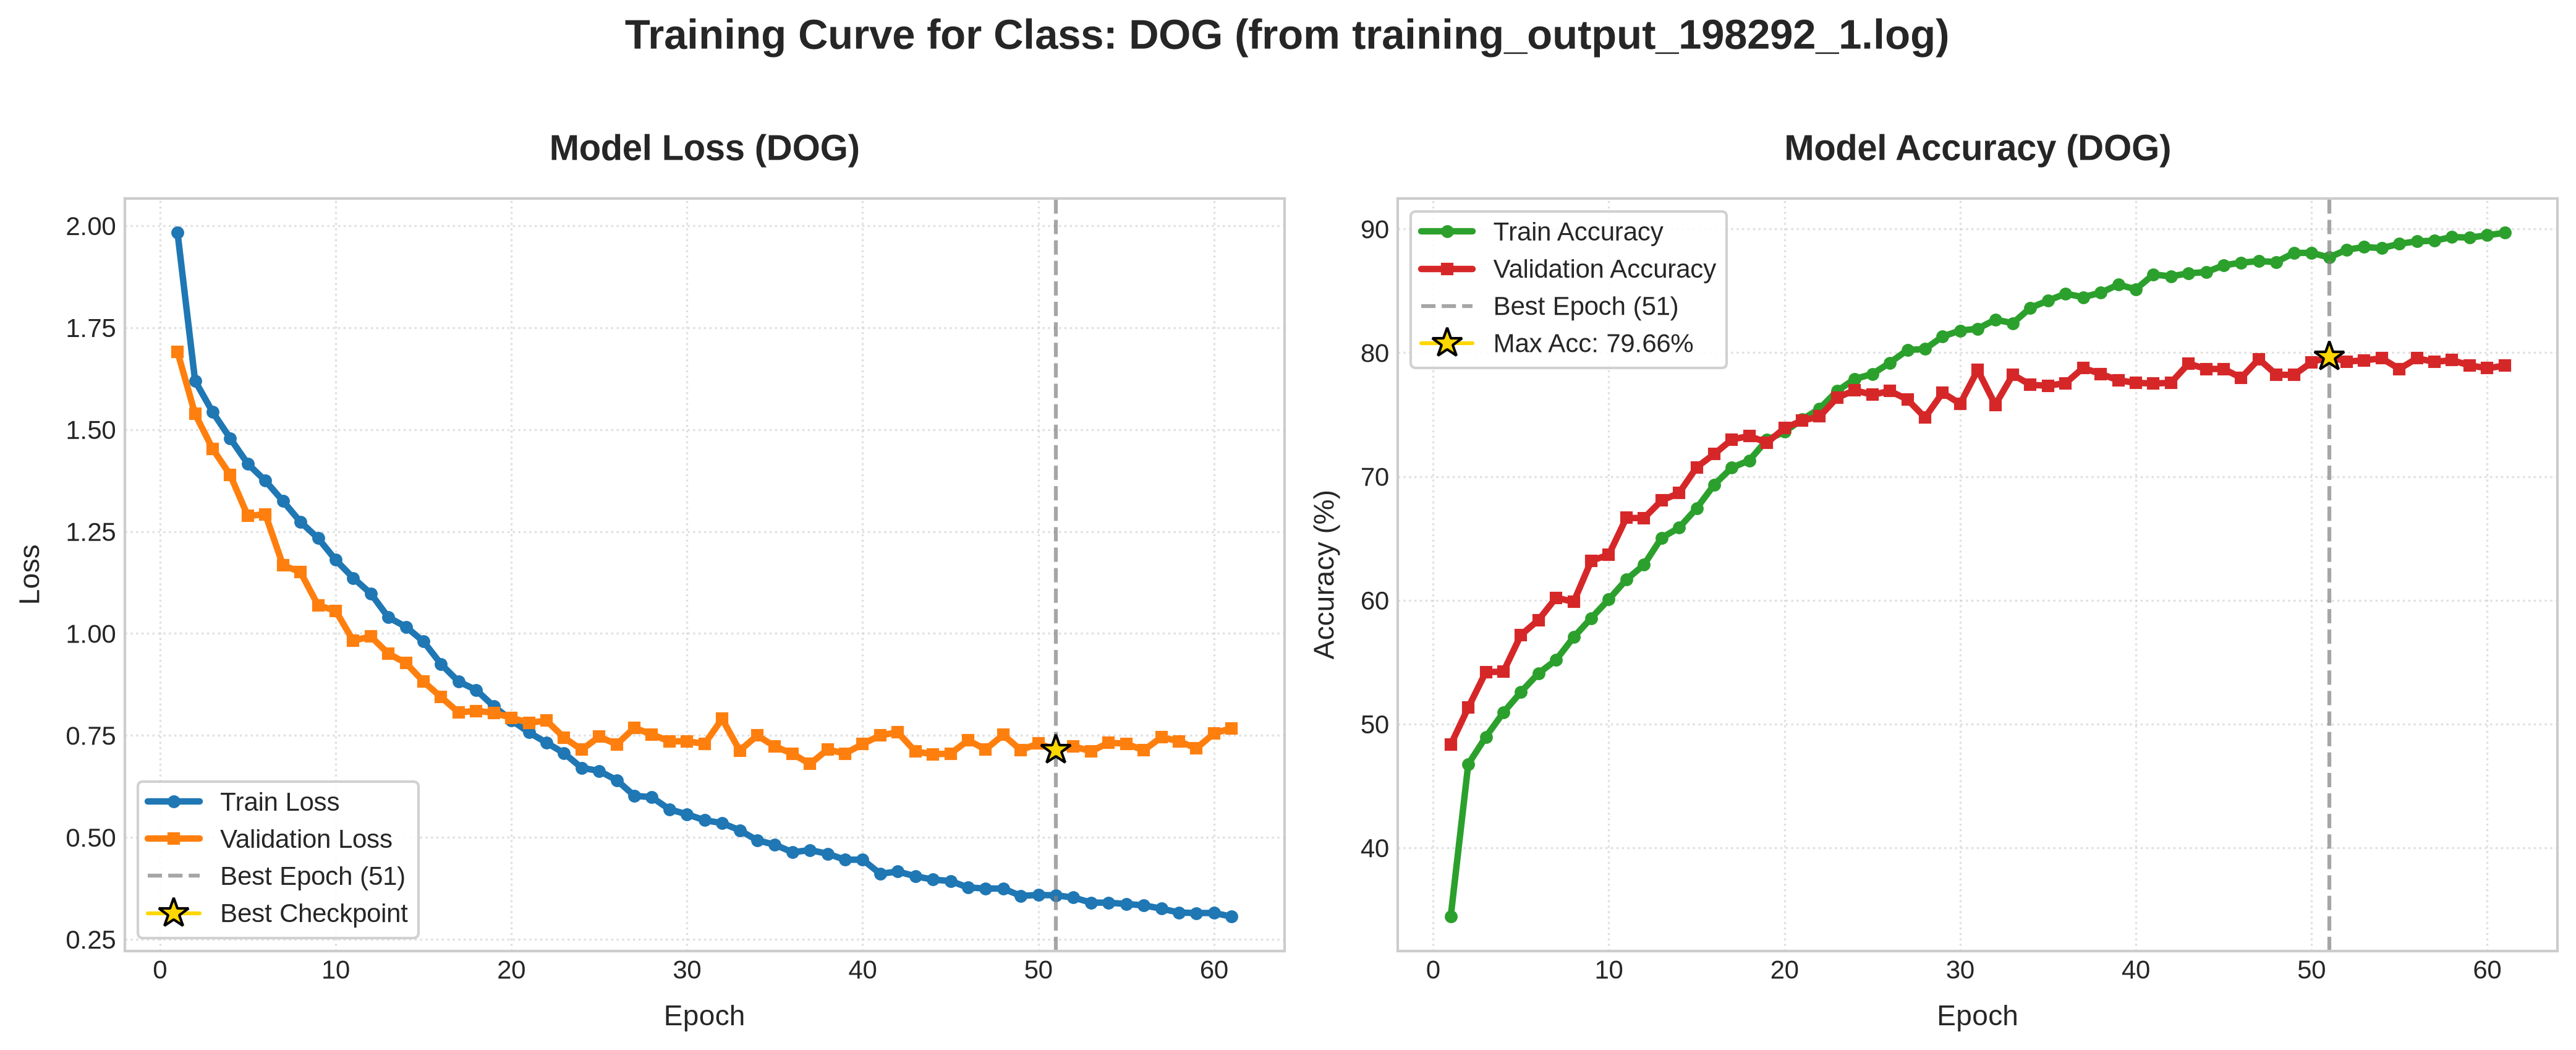
\includegraphics[width=\textwidth]{../Epoch/loss_Graphs/training_output_198292_1_dog.png}
        \caption{Task 1: Dog Baseline ($\text{LR}=1\times 10^{-5}$, 100 Ep.)}
    \end{subfigure}
    \hfill
    \begin{subfigure}[b]{0.48\textwidth}
        \centering
        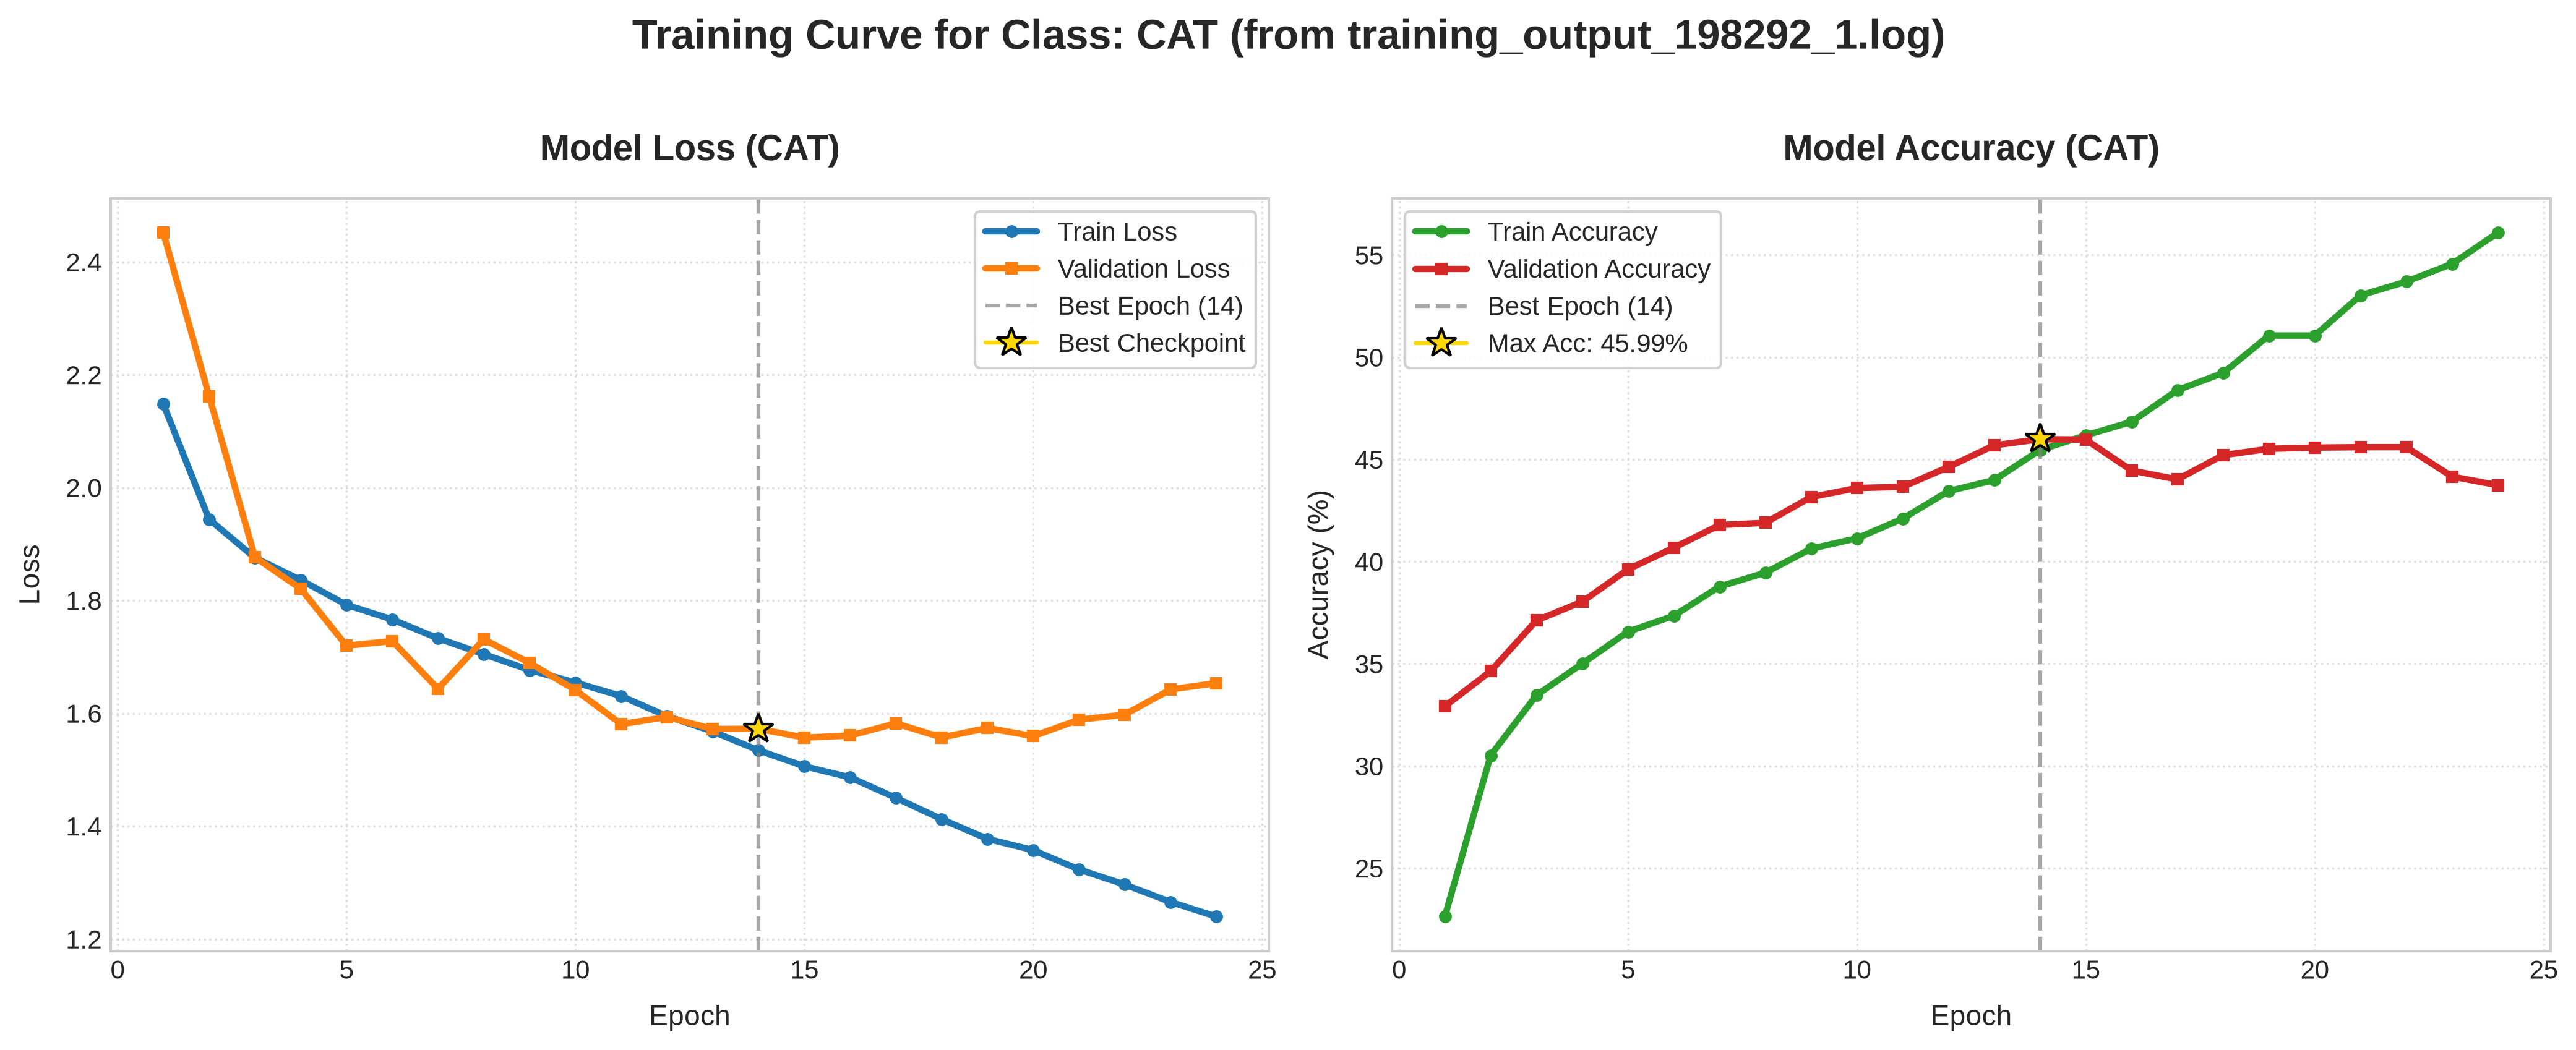
\includegraphics[width=\textwidth]{../Epoch/loss_Graphs/training_output_198292_1_cat.png}
        \caption{Task 1: Cat Baseline ($\text{LR}=1\times 10^{-5}$, 100 Ep.)}
    \end{subfigure}
    
    \vspace{0.3cm}
    
    % Task 2: Balanced Weights
    \begin{subfigure}[b]{0.48\textwidth}
        \centering
        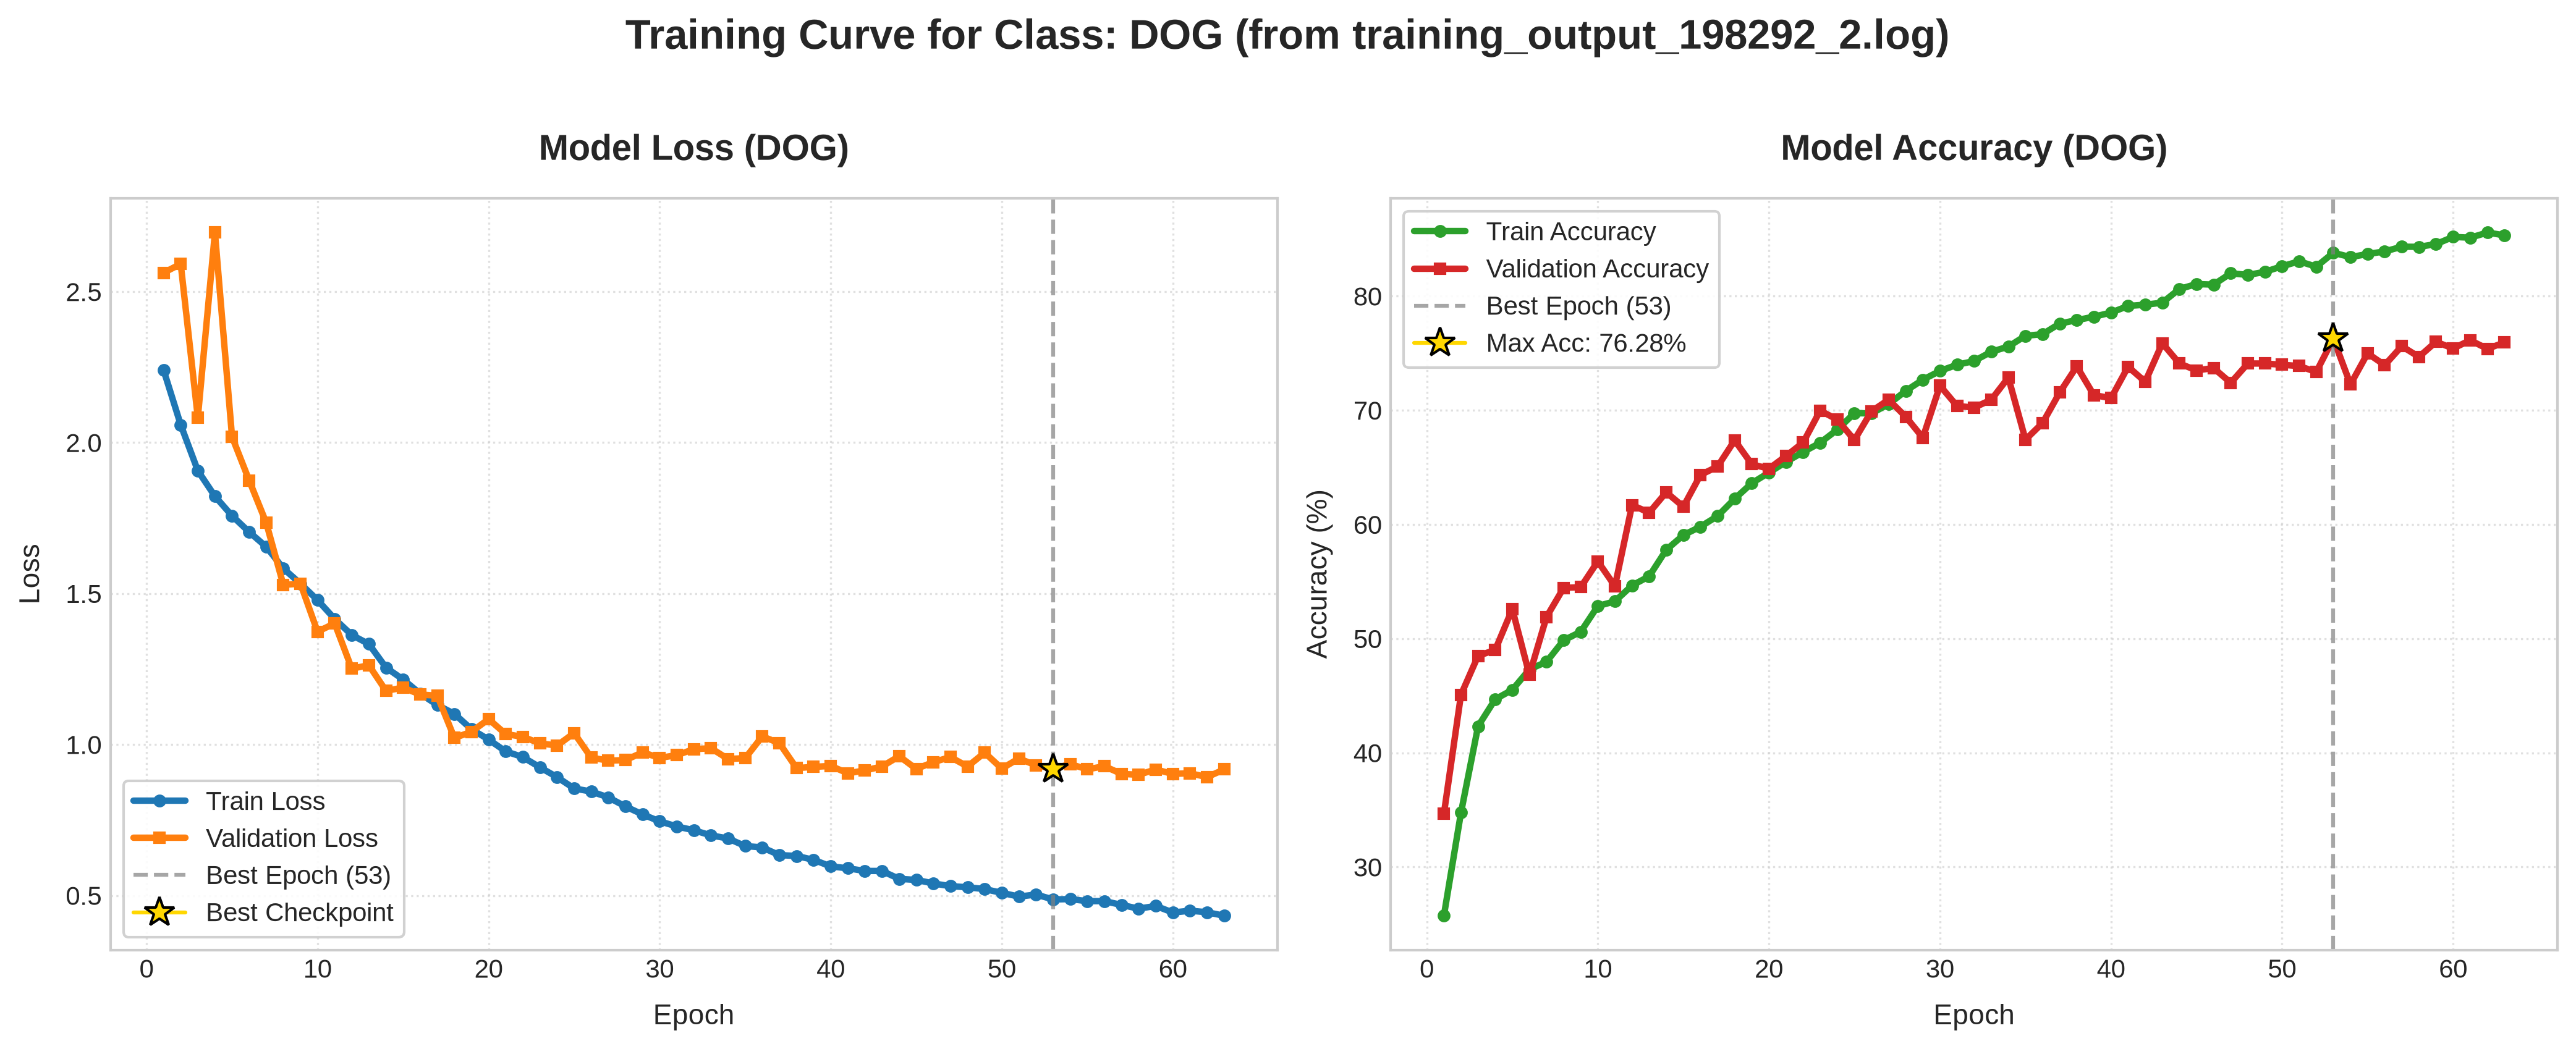
\includegraphics[width=\textwidth]{../Epoch/loss_Graphs/training_output_198292_2_dog.png}
        \caption{Task 2: Dog Balanced Weights ($\text{LR}=1\times 10^{-5}$, 100 Ep.)}
    \end{subfigure}
    \hfill
    \begin{subfigure}[b]{0.48\textwidth}
        \centering
        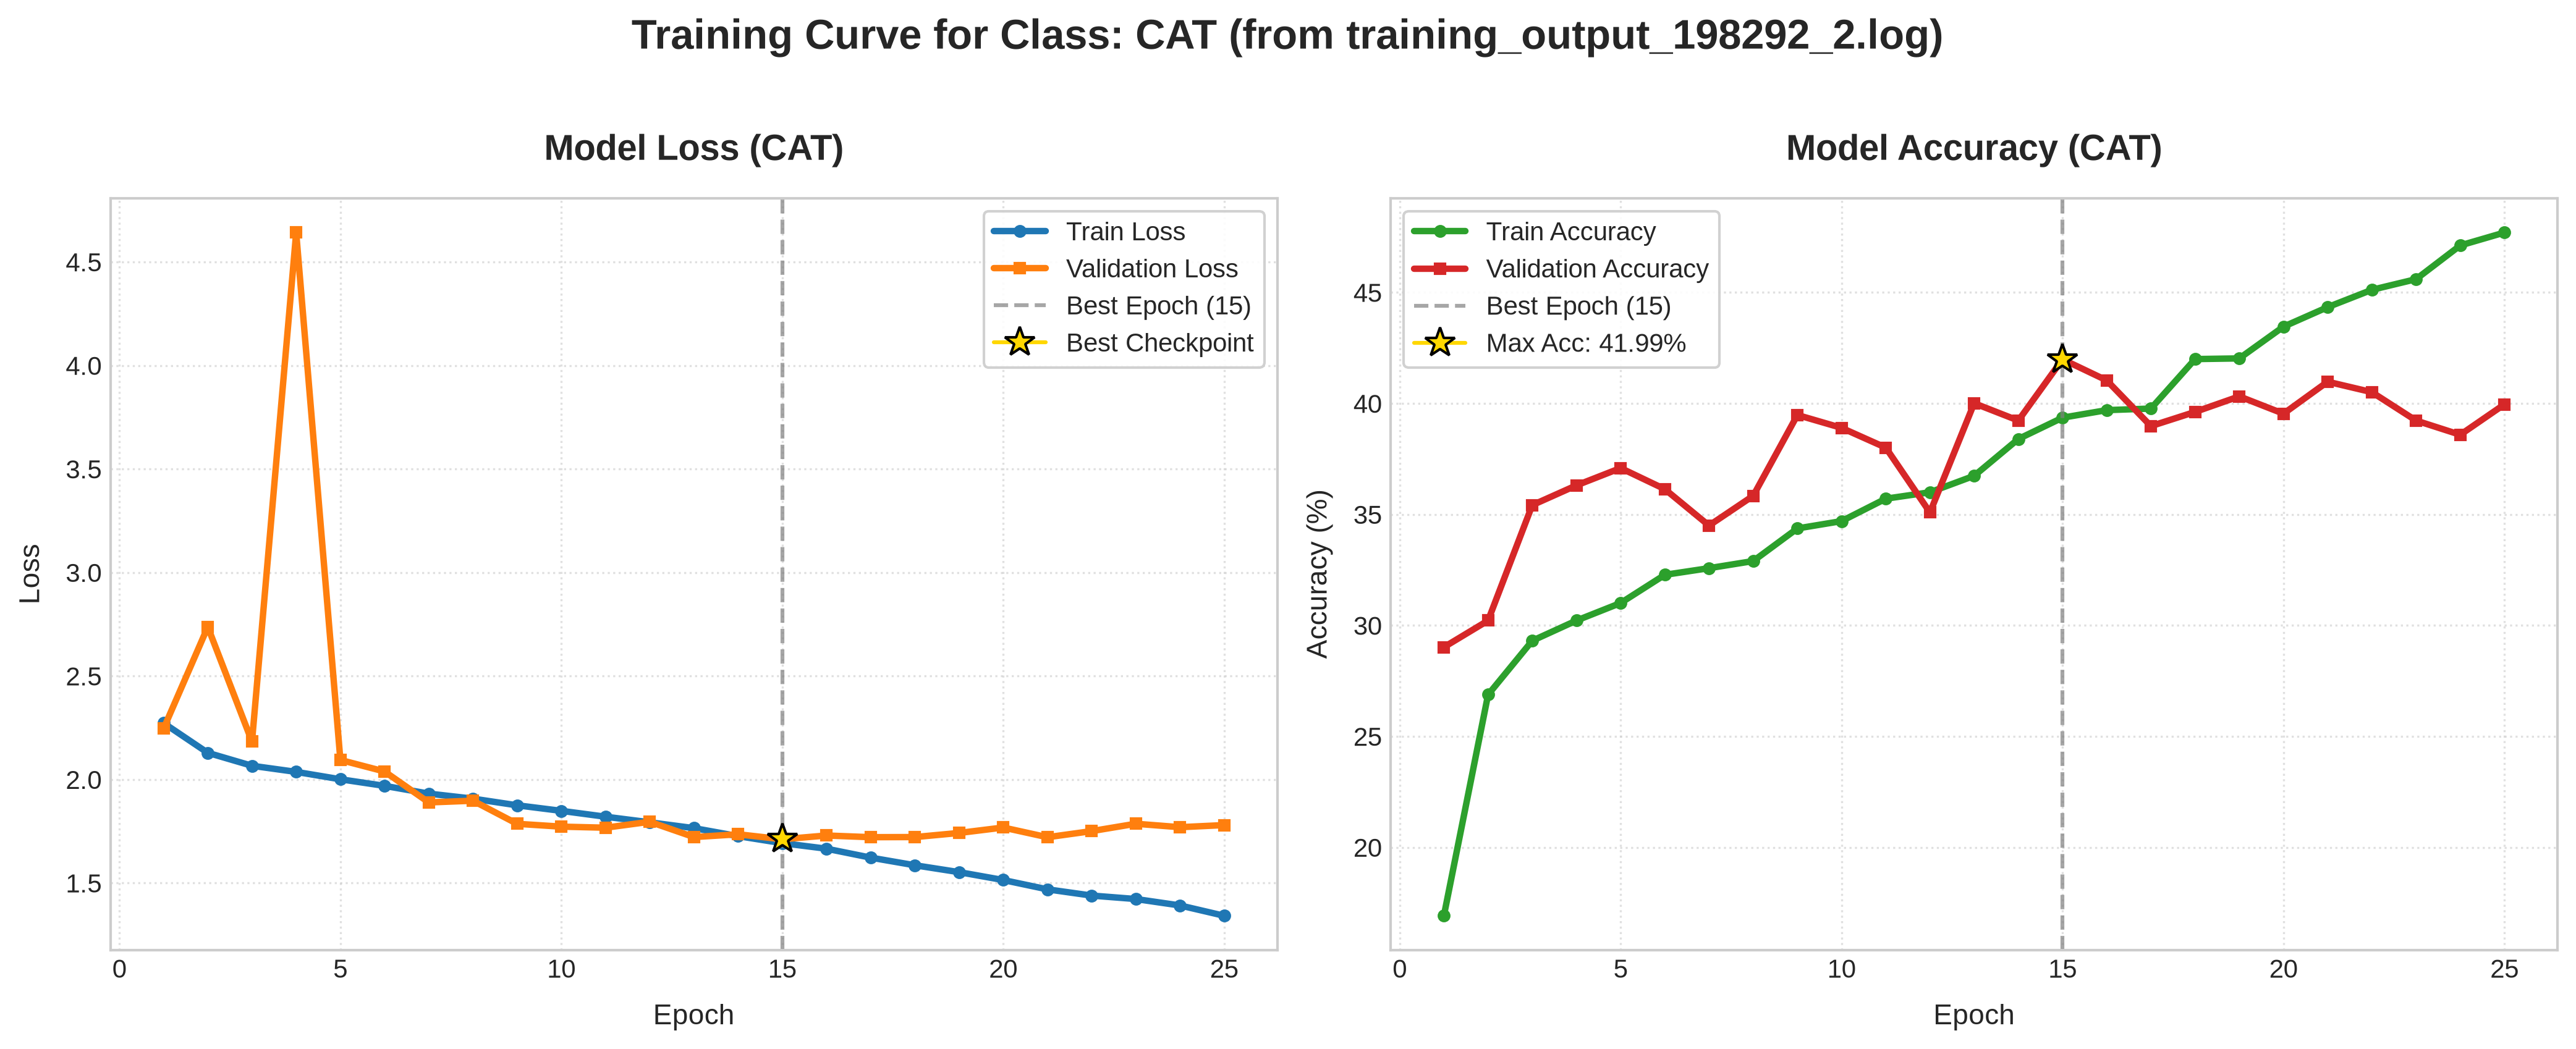
\includegraphics[width=\textwidth]{../Epoch/loss_Graphs/training_output_198292_2_cat.png}
        \caption{Task 2: Cat Balanced Weights ($\text{LR}=1\times 10^{-5}$, 100 Ep.)}
    \end{subfigure}

    \vspace{0.3cm}

    % Task 3: Blur
    \begin{subfigure}[b]{0.48\textwidth}
        \centering
        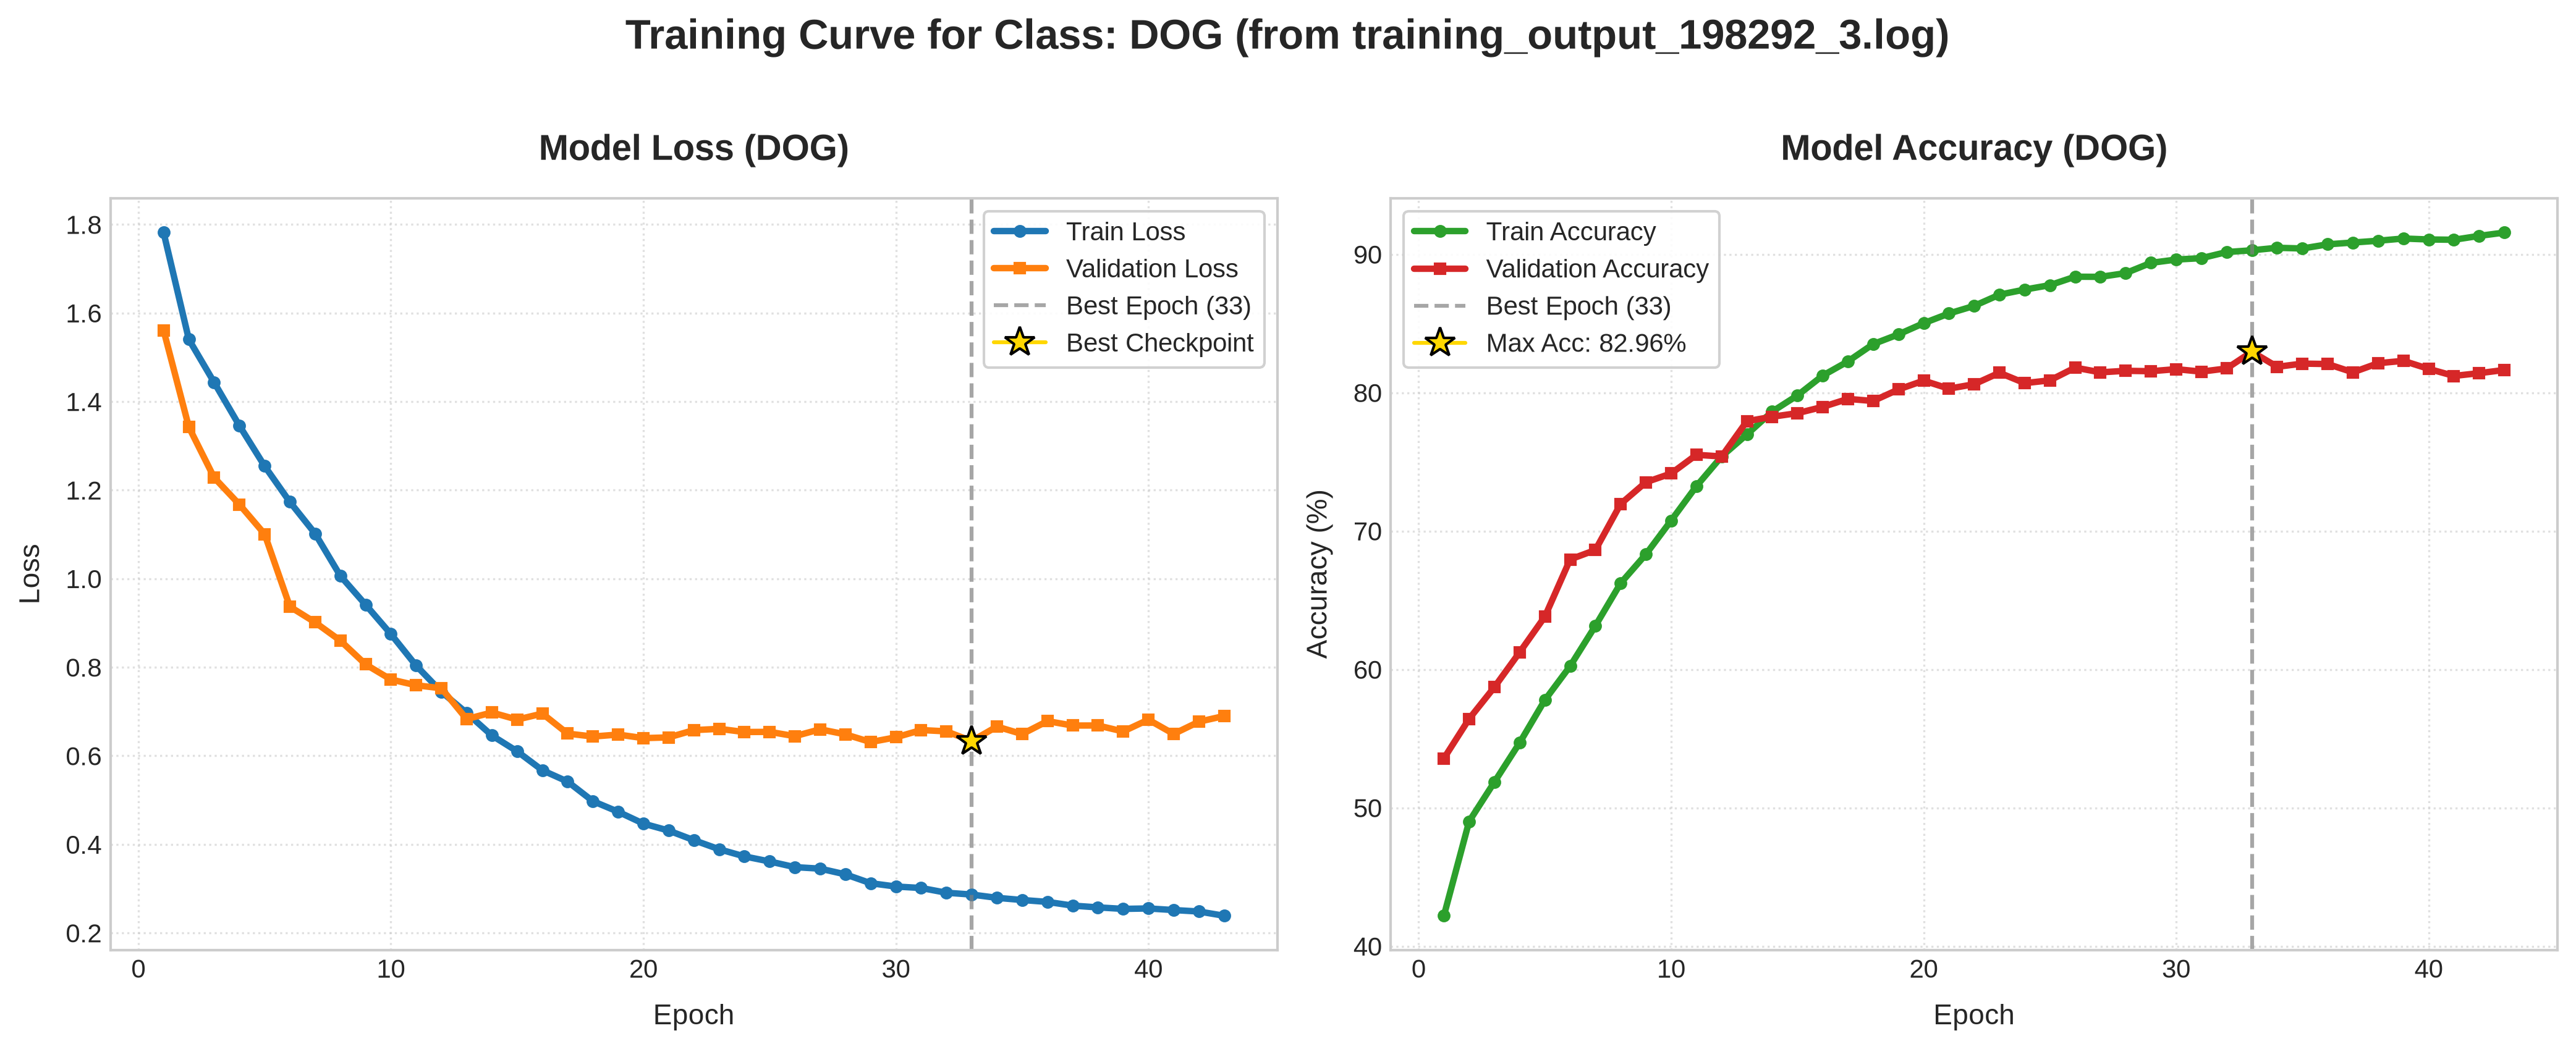
\includegraphics[width=\textwidth]{../Epoch/loss_Graphs/training_output_198292_3_dog.png}
        \caption{Task 3: Dog Blur ($\text{LR}=1\times 10^{-5}$, 100 Ep., $82.96\%$)}
    \end{subfigure}
    \hfill
    \begin{subfigure}[b]{0.48\textwidth}
        \centering
        \includegraphics[width=\textwidth]{../Epoch/loss_Graphs/training_output_198292_3_cat.png}
        \caption{Task 3: Cat Blur ($\text{LR}=1\times 10^{-5}$, 100 Ep., $47.13\%$)}
    \end{subfigure}

    \vspace{0.3cm}

    % Task 4: Mirror
    \begin{subfigure}[b]{0.48\textwidth}
        \centering
        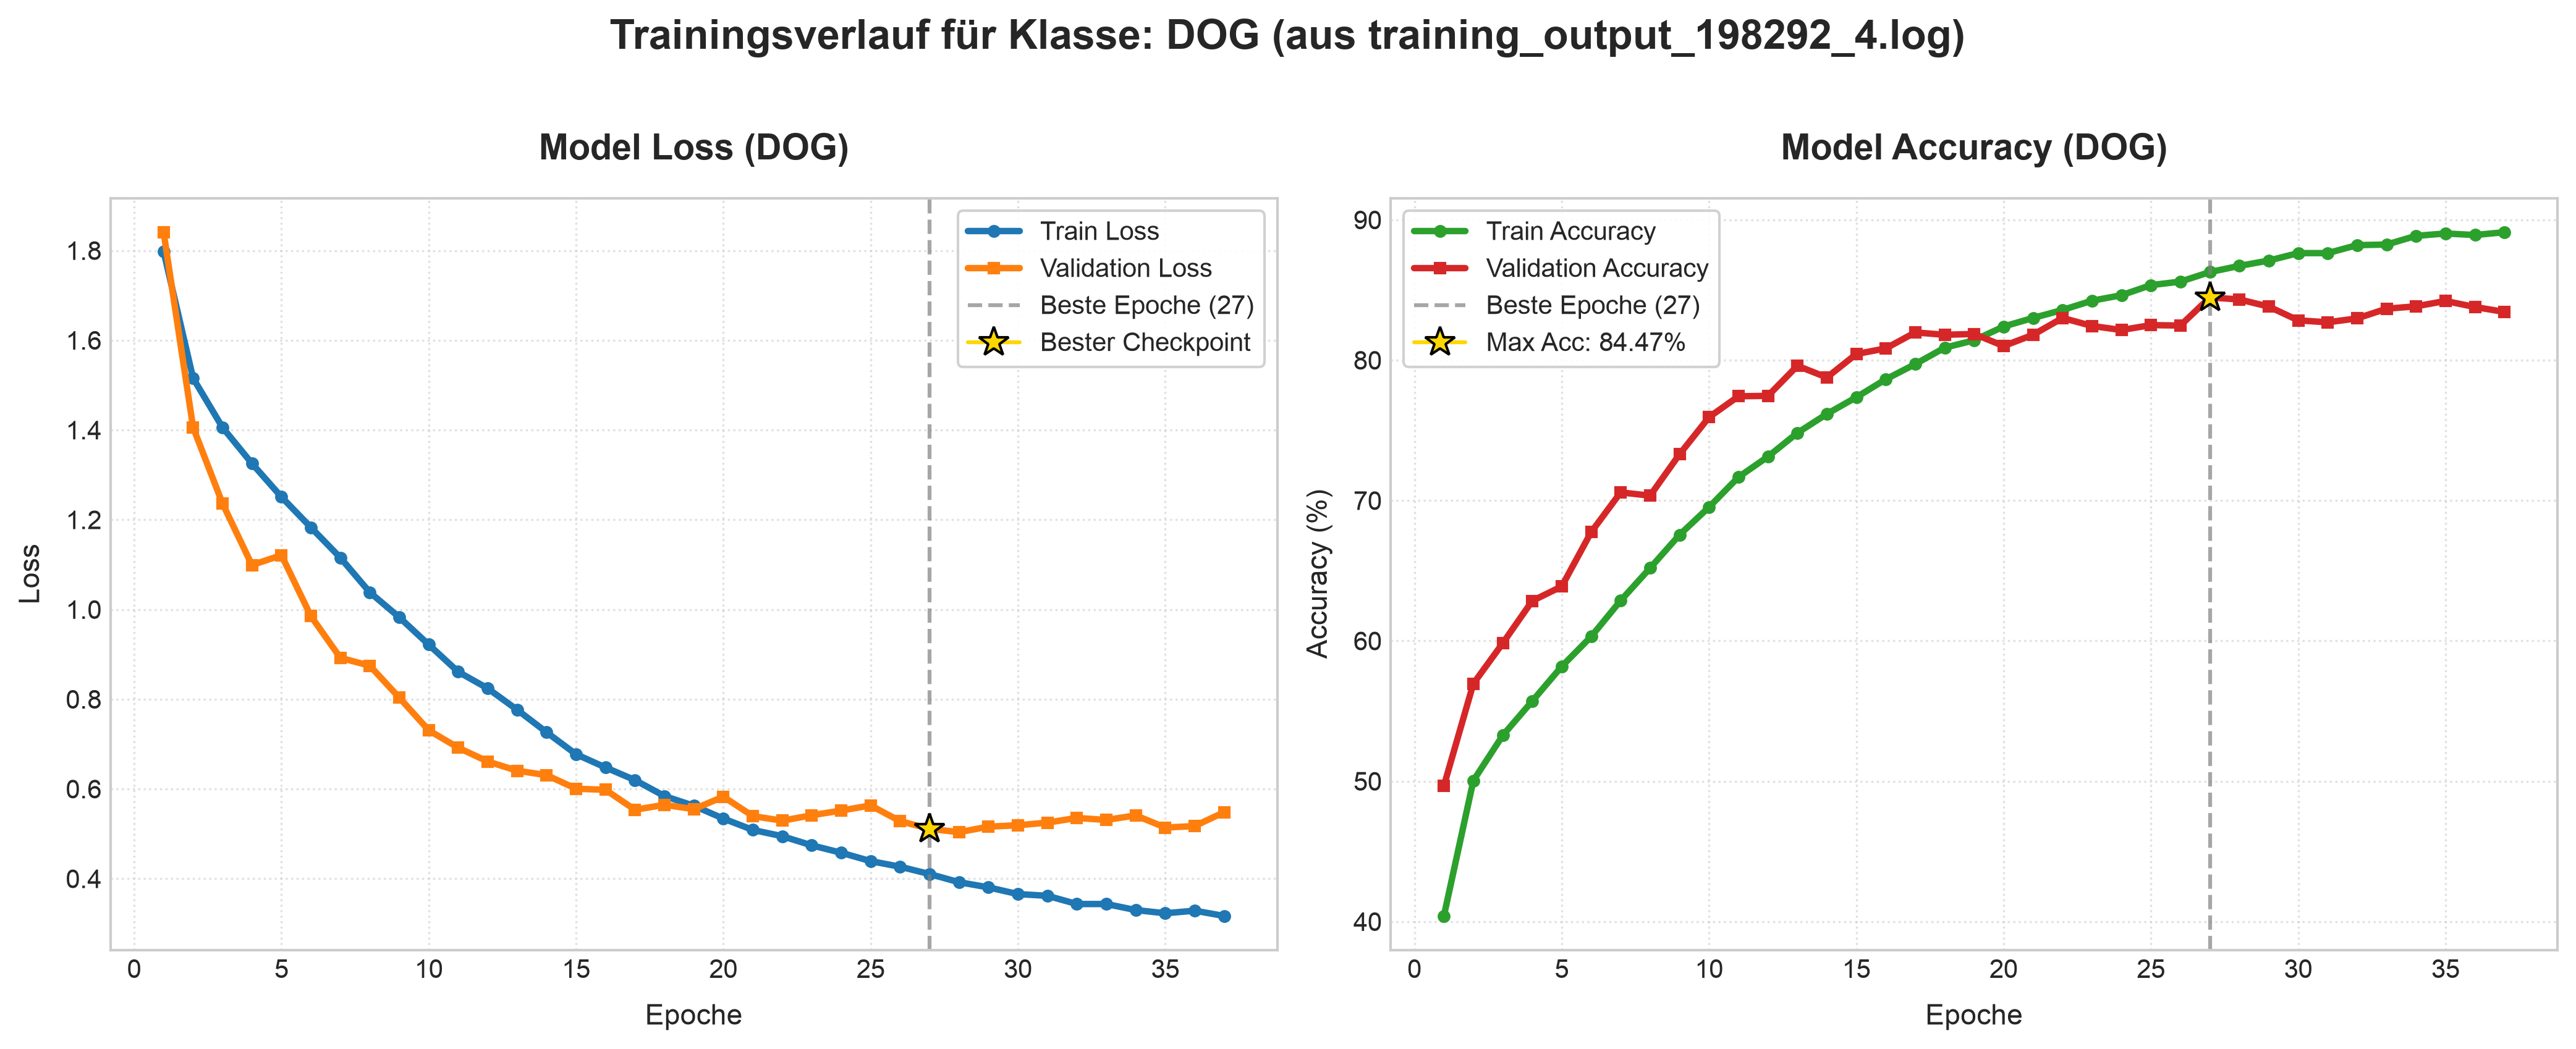
\includegraphics[width=\textwidth]{../Epoch/loss_Graphs/training_output_198292_4_dog.png}
        \caption{Task 4: Dog Mirror ($\text{LR}=1\times 10^{-5}$, 100 Ep.)}
    \end{subfigure}
    \hfill
    \begin{subfigure}[b]{0.48\textwidth}
        \centering
        \includegraphics[width=\textwidth]{../Epoch/loss_Graphs/training_output_198292_4_cat.png}
        \caption{Task 4: Cat Mirror ($\text{LR}=1\times 10^{-5}$, 100 Ep., $49.89\%$)}
    \end{subfigure}

    \vspace{0.3cm}

    % Task 5: CropMix
    \begin{subfigure}[b]{0.48\textwidth}
        \centering
        \includegraphics[width=\textwidth]{../Epoch/loss_Graphs/training_output_198292_5_dog.png}
        \caption{Task 5: Dog CropMix ($\text{LR}=1\times 10^{-5}$, 100 Ep., $84.99\%$)}
    \end{subfigure}
    \hfill
    \begin{subfigure}[b]{0.48\textwidth}
        \centering
        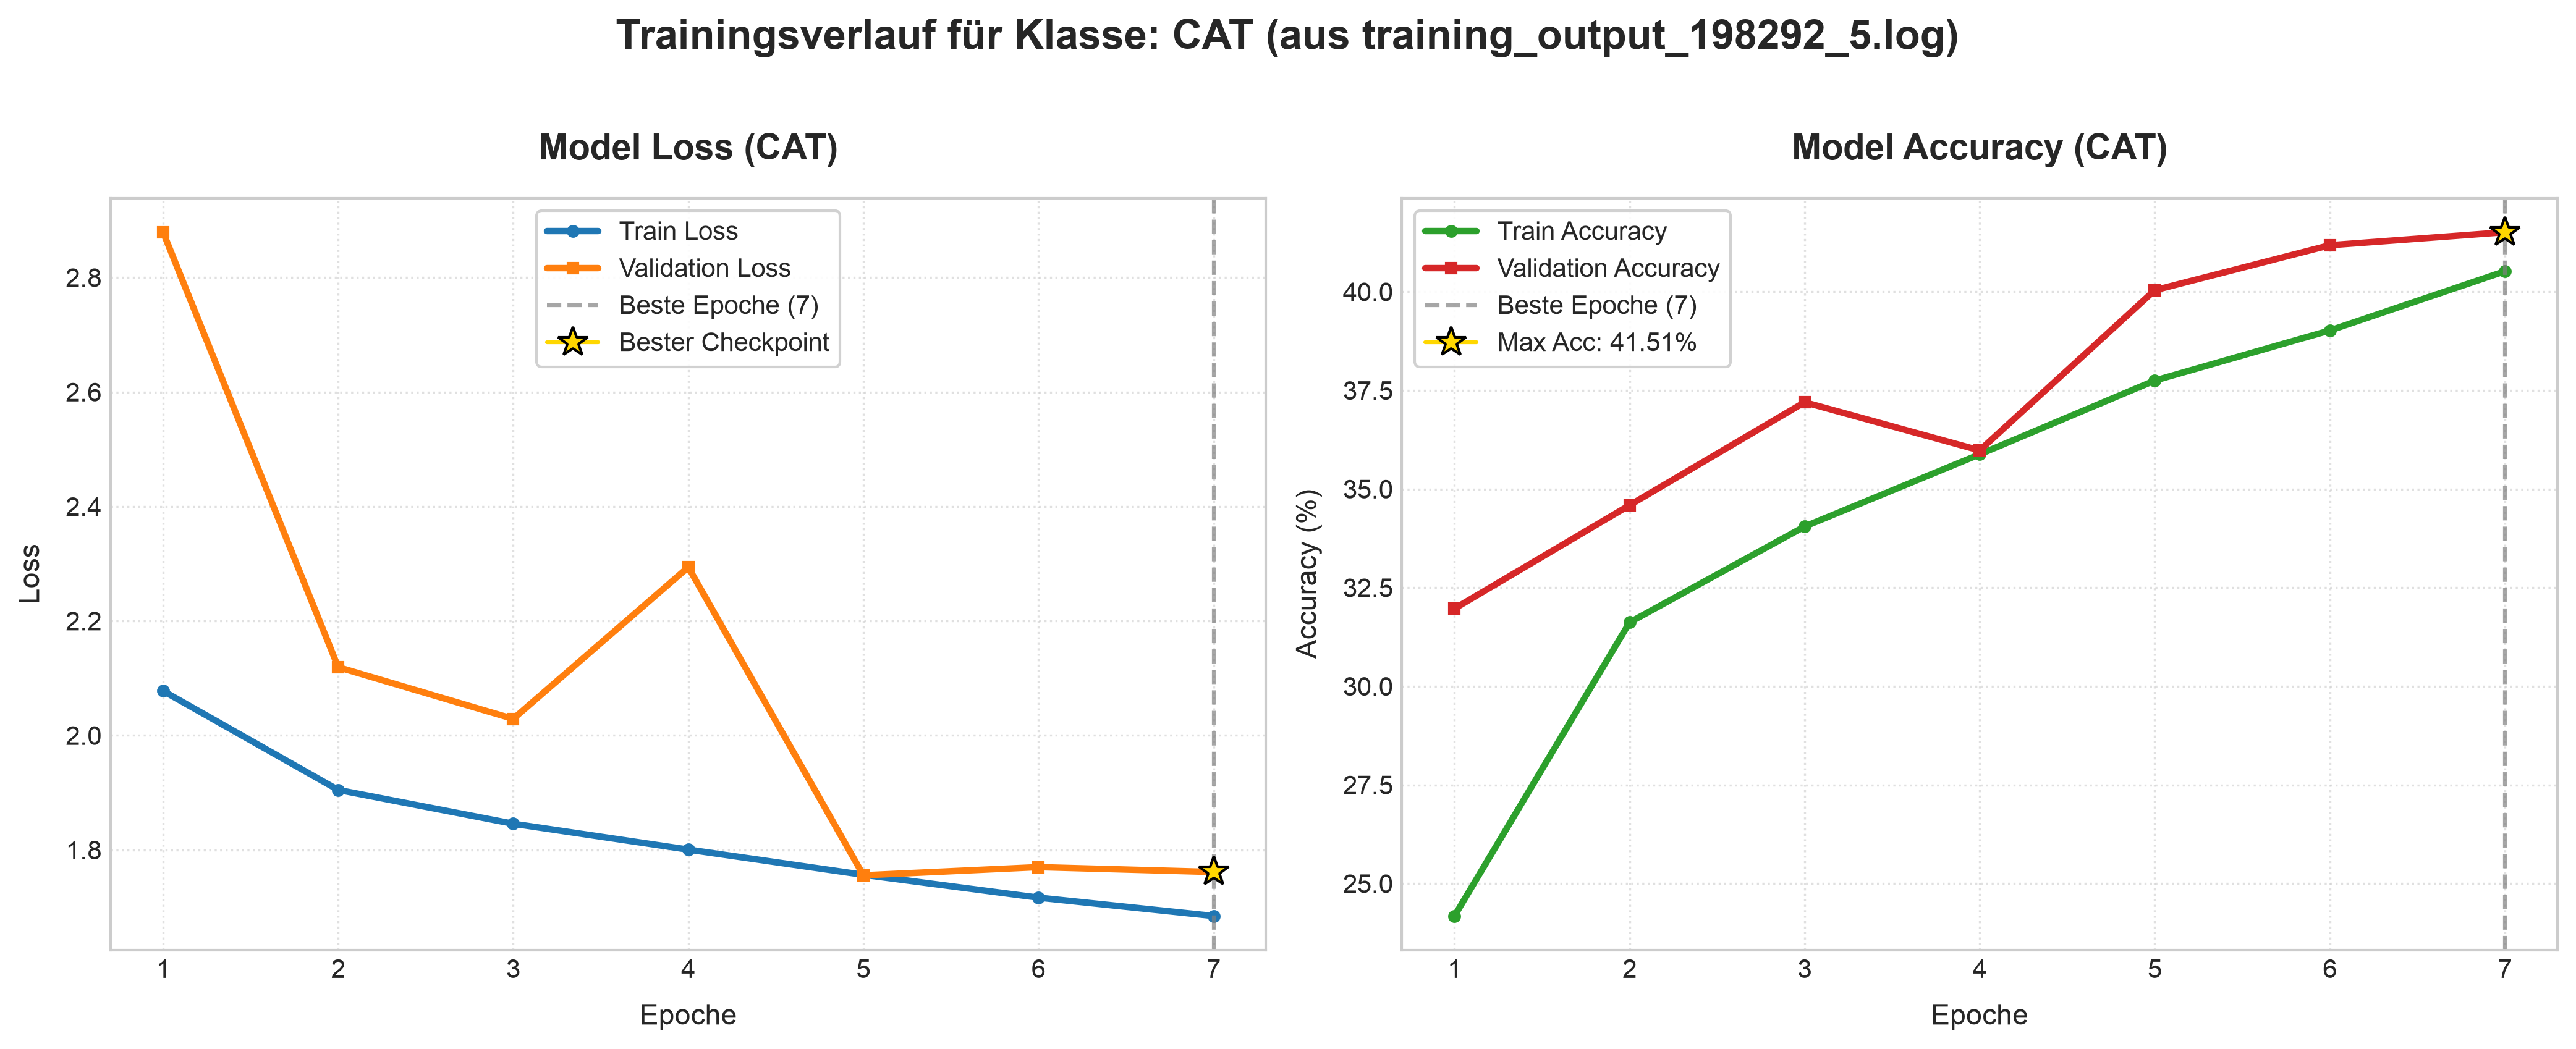
\includegraphics[width=\textwidth]{../Epoch/loss_Graphs/training_output_198292_5_cat.png}
        \caption{Task 5: Cat CropMix ($\text{LR}=1\times 10^{-5}$, 100 Ep.)}
    \end{subfigure}

    \vspace{0.3cm}

    % Task 6: All Augmentations Combined
    \begin{subfigure}[b]{0.48\textwidth}
        \centering
        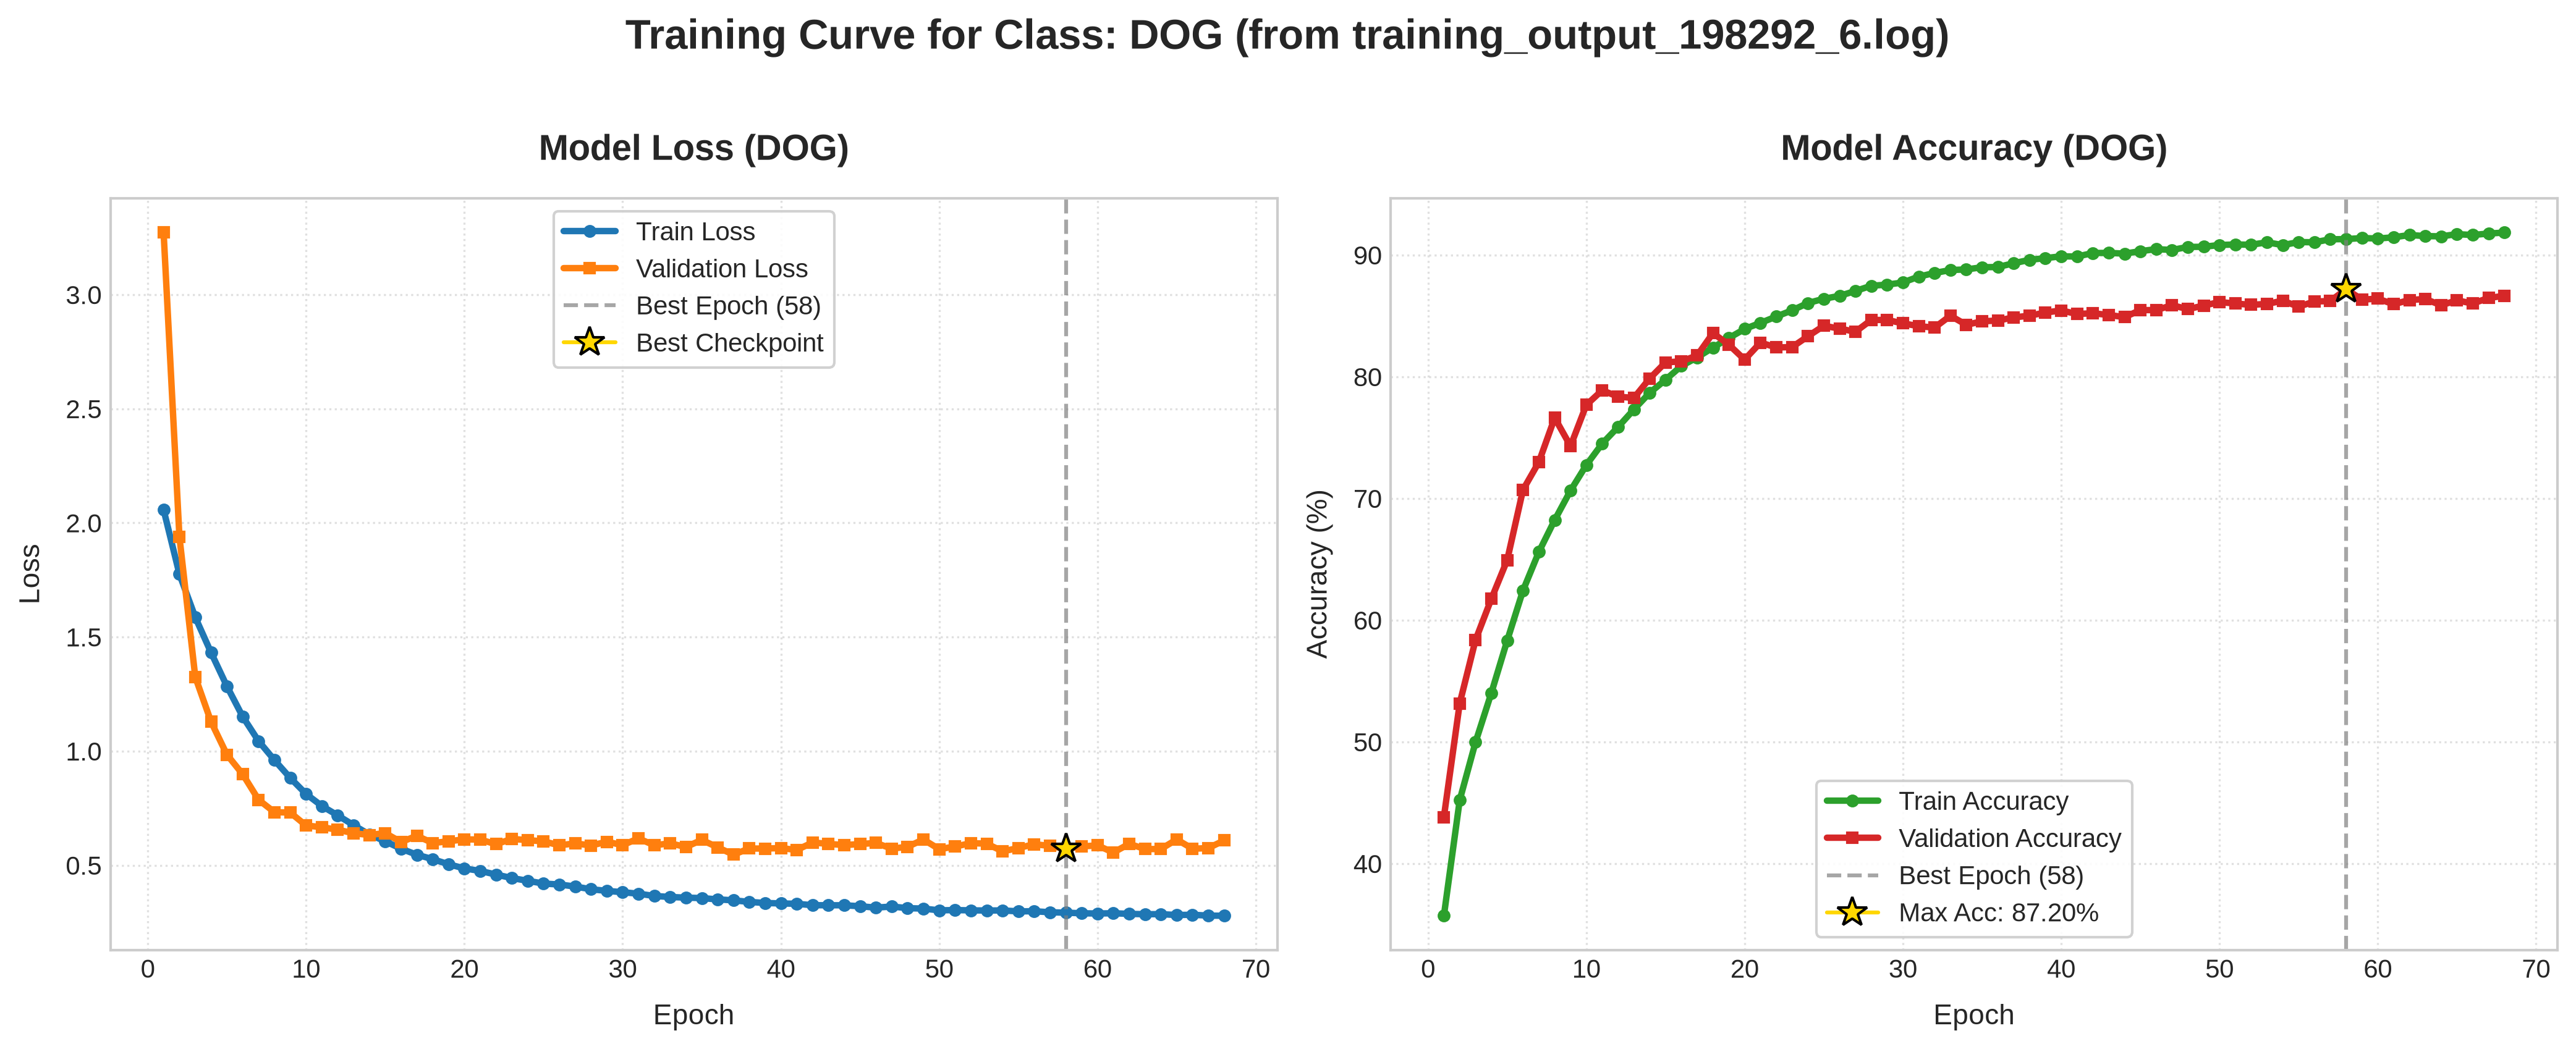
\includegraphics[width=\textwidth]{../Epoch/loss_Graphs/training_output_198292_6_dog.png}
        \caption{Task 6: Dog All Augs ($\text{LR}=1\times 10^{-5}$, 100 Ep.)}
    \end{subfigure}
    \hfill
    \begin{subfigure}[b]{0.48\textwidth}
        \centering
        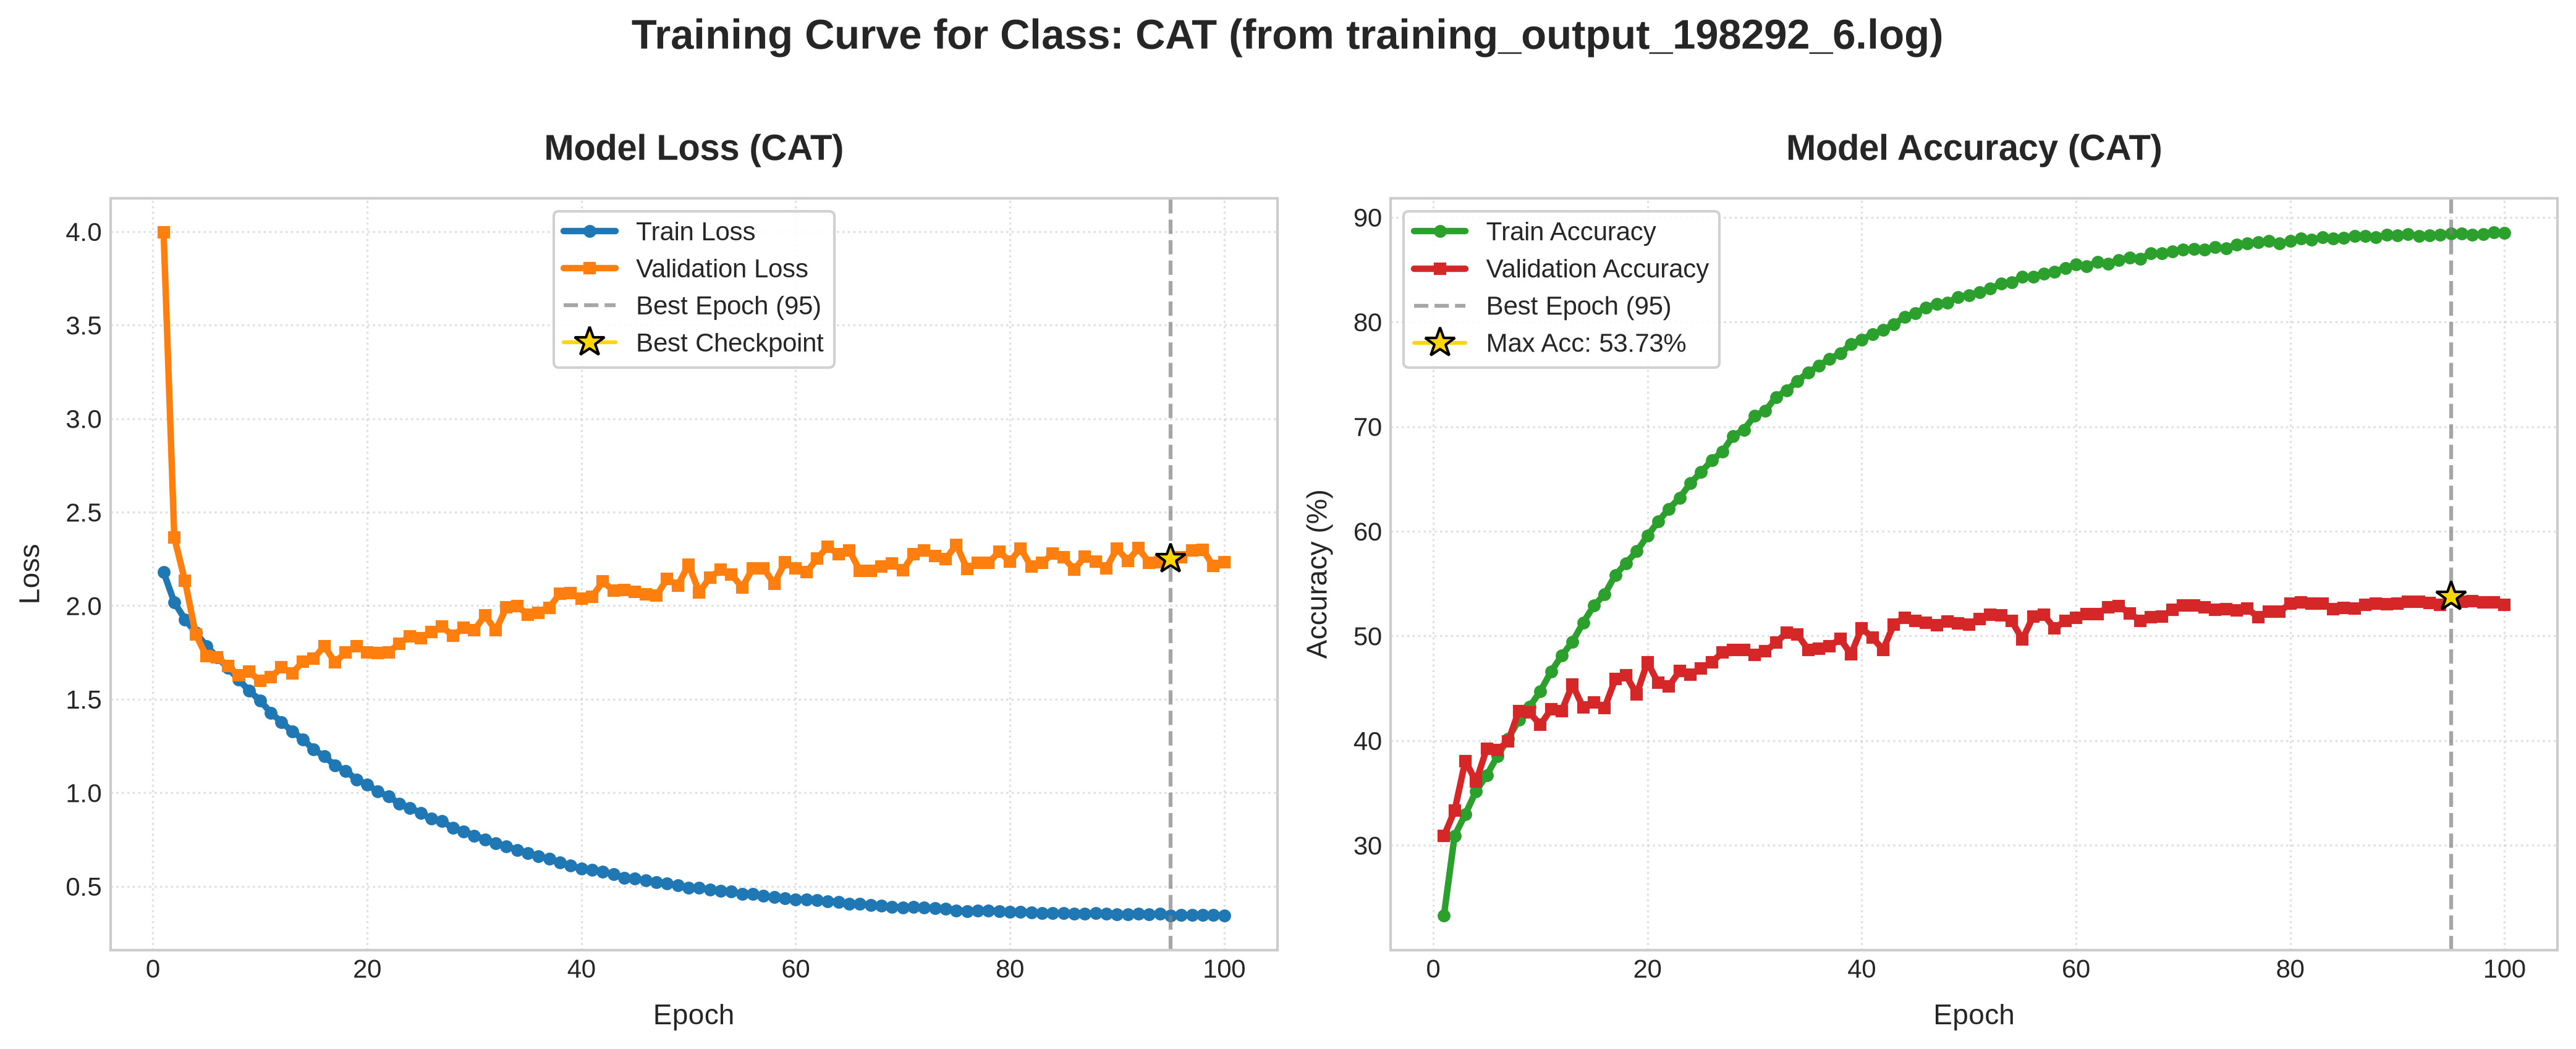
\includegraphics[width=\textwidth]{../Epoch/loss_Graphs/training_output_198292_6_cat.png}
        \caption{Task 6: Cat All Augs ($\text{LR}=1\times 10^{-5}$, 100 Ep., $53.73\%$)}
    \end{subfigure}

    \vspace{0.3cm}

    % Task 7: Long Run Baseline
    \begin{subfigure}[b]{0.48\textwidth}
        \centering
        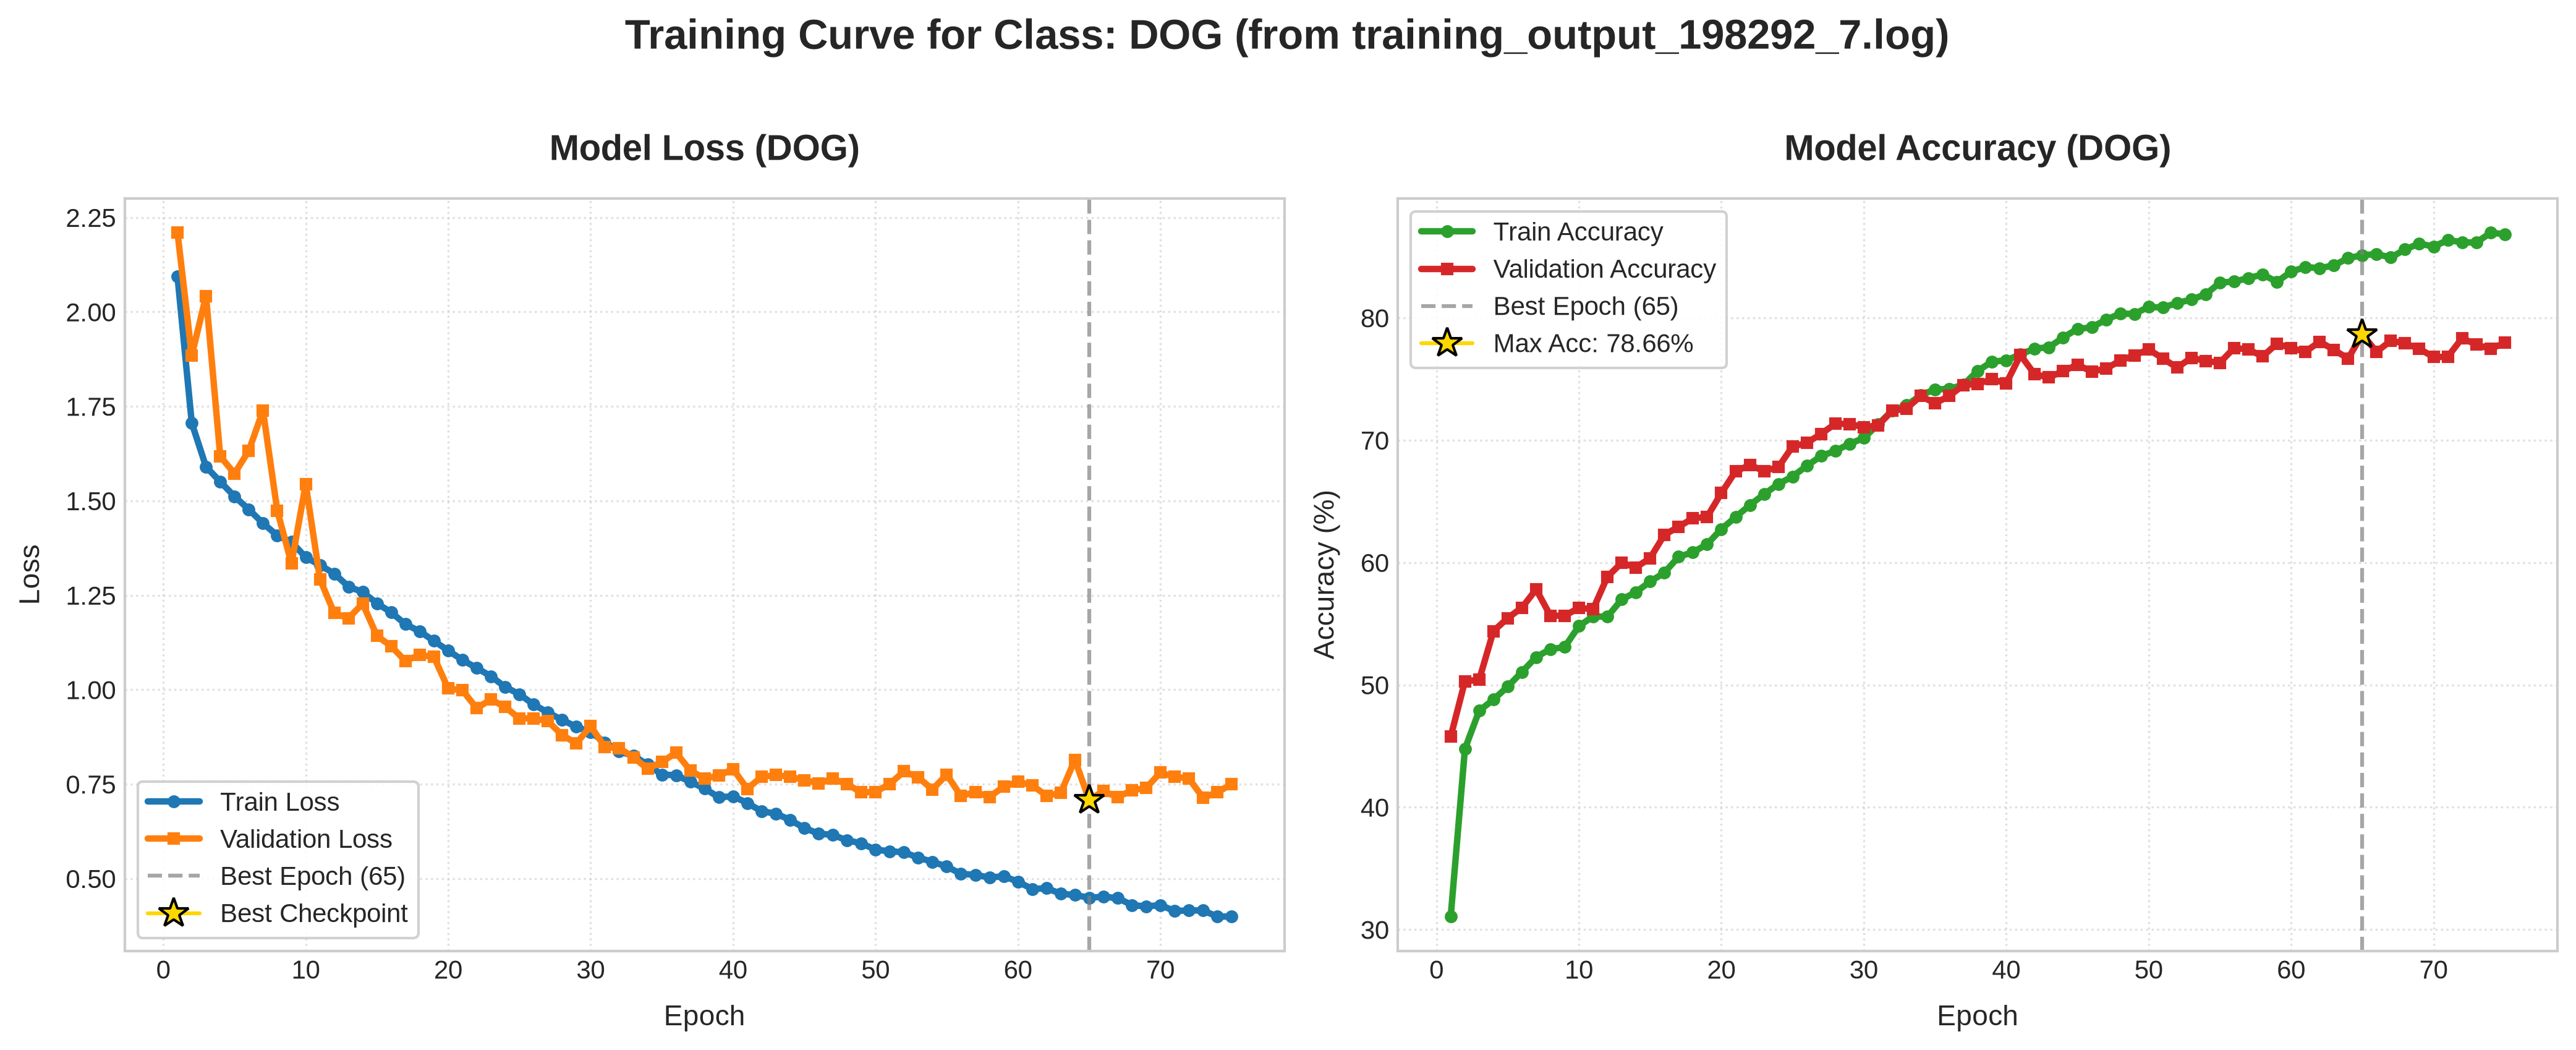
\includegraphics[width=\textwidth]{../Epoch/loss_Graphs/training_output_198292_7_dog.png}
        \caption{Task 7: Dog Extended Baseline ($\text{LR}=5\times 10^{-6}$, 1000 Ep., $78.66\%$)}
    \end{subfigure}
    \hfill
    \begin{subfigure}[b]{0.48\textwidth}
        \centering
        \includegraphics[width=\textwidth]{../Epoch/loss_Graphs/training_output_198292_7_cat.png}
        \caption{Task 7: Cat Extended Baseline ($\text{LR}=5\times 10^{-6}$, 1000 Ep., $46.13\%$)}
    \end{subfigure}
    
    \caption{Comprehensive comparison of training loss and accuracy dynamics across all Cat and Dog classification runs (Tasks 1--7) under various augmentation strategies and learning rates (all models trained from uninitialized weights).}
    \label{fig:appendix_training_curves}
\end{figure*}

\section{Detailed Training History Curves}
\label{sec:appendix_curves}

This appendix presents the full training and validation loss alongside accuracy progression curves across all seven experimental configurations for both Cat and Dog datasets.

\begin{figure*}[htbp]
    \centering
    \begin{subfigure}[b]{0.48\textwidth}
        \centering
        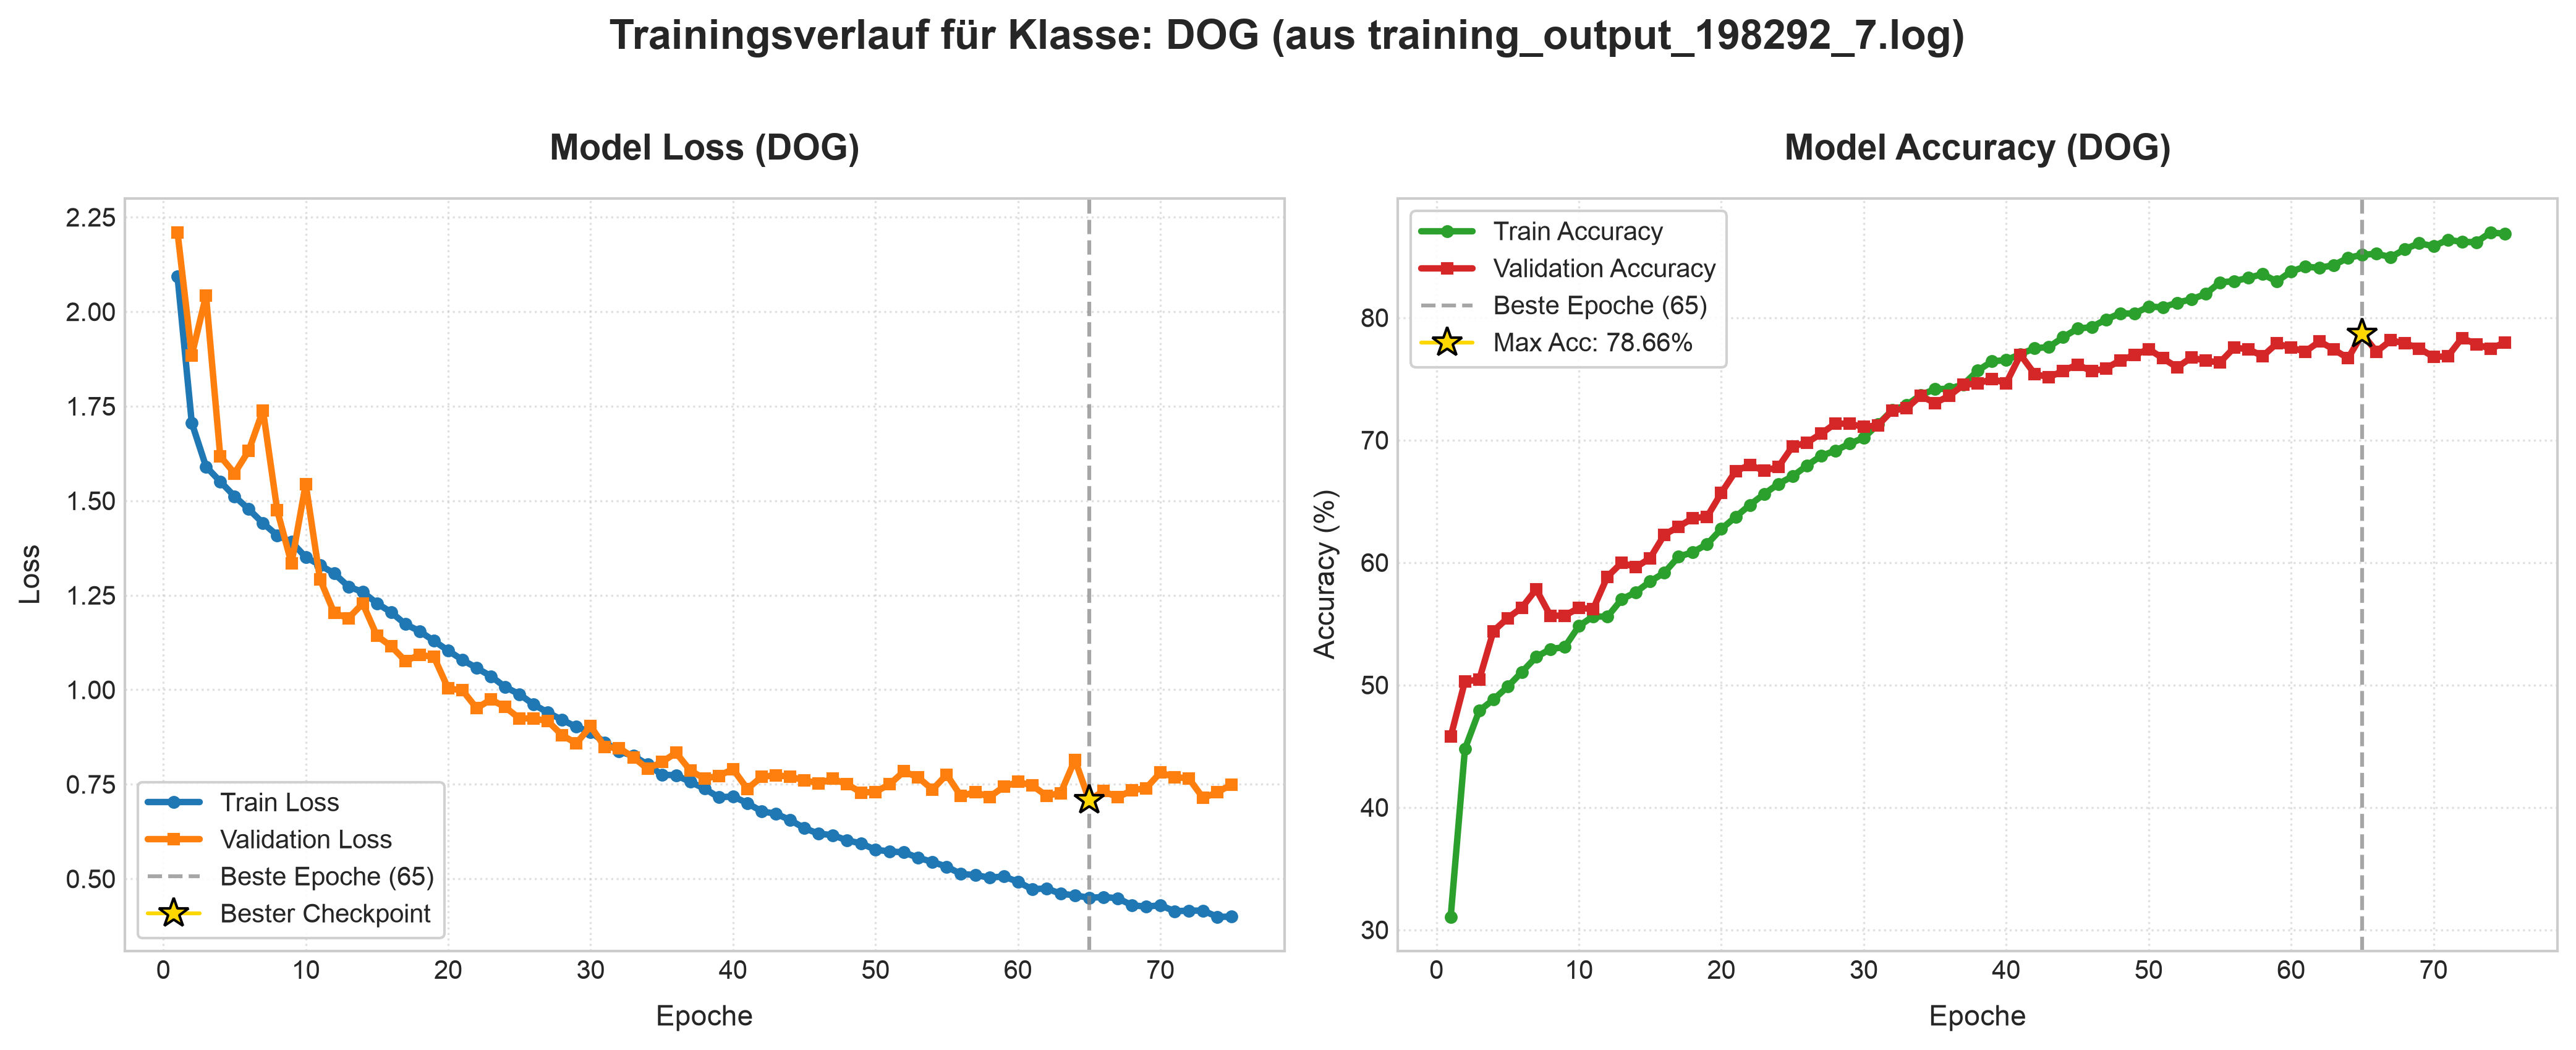
\includegraphics[width=\textwidth]{../L_A_Graphs/training_output_198292_7_dog.png}
        \caption{Task 7: Dog Baseline ($78.66\%$)}
    \end{subfigure}
    \hfill
    \begin{subfigure}[b]{0.48\textwidth}
        \centering
        \includegraphics[width=\textwidth]{../L_A_Graphs/training_output_198292_7_cat.png}
        \caption{Task 7: Cat Baseline ($46.13\%$)}
    \end{subfigure}
    
    \vspace{0.3cm}
    
    \begin{subfigure}[b]{0.48\textwidth}
        \centering
        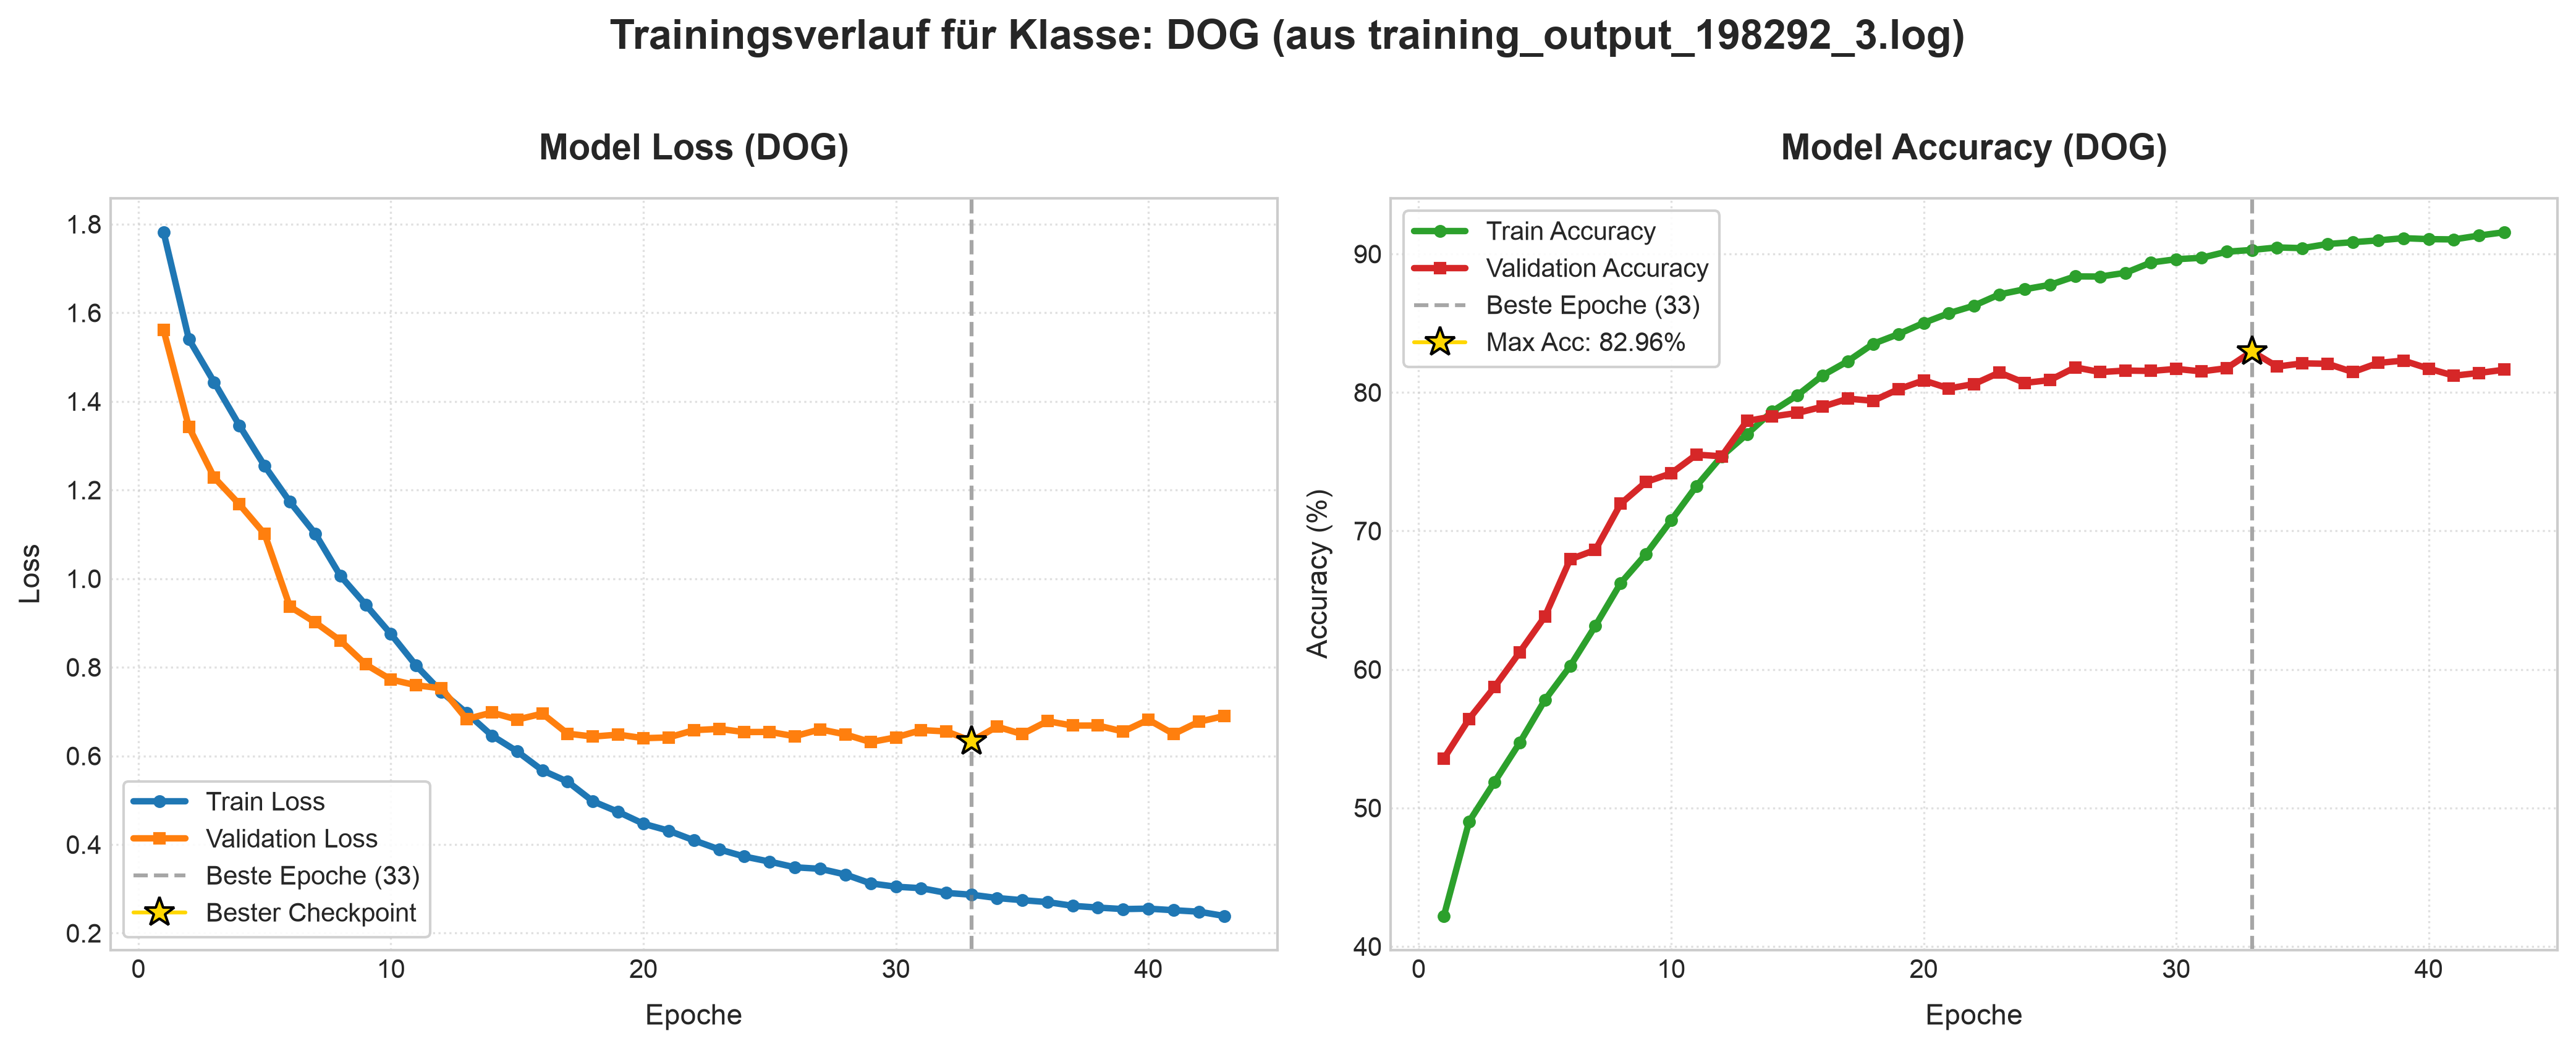
\includegraphics[width=\textwidth]{../L_A_Graphs/training_output_198292_3_dog.png}
        \caption{Task 3: Dog Blur ($82.96\%$)}
    \end{subfigure}
    \hfill
    \begin{subfigure}[b]{0.48\textwidth}
        \centering
        \includegraphics[width=\textwidth]{../L_A_Graphs/training_output_198292_3_cat.png}
        \caption{Task 3: Cat Blur ($47.13\%$)}
    \end{subfigure}

    \vspace{0.3cm}
    
    \begin{subfigure}[b]{0.48\textwidth}
        \centering
        \includegraphics[width=\textwidth]{../L_A_Graphs/training_output_198292_5_dog.png}
        \caption{Task 5: Dog CropMix ($84.99\%$)}
    \end{subfigure}
    \hfill
    \begin{subfigure}[b]{0.48\textwidth}
        \centering
        \includegraphics[width=\textwidth]{../L_A_Graphs/training_output_198292_4_cat.png}
        \caption{Task 4: Cat Mirror ($49.89\%$)}
    \end{subfigure}
    
    \caption{Comparison of training loss and accuracy dynamics across Cat and Dog classification runs under different augmentation strategies when trained from uninitialized weights.}
    \label{fig:appendix_training_curves}
\end{figure*}
% supplementary material
% \input{sec/X_suppl}

\end{document}
